\chapter{Attacks}
\label{chp:attacks}
After giving an overview of the dataset and model, which we use as a basis for our following experiments, we will now define our proposed targeted item-to-item attacks and discuss our experimental results against an undefended visual \acl{RS}, as described in Chapter~\ref{chp:model}.

\section{Adversary Model}
\label{sec:adv-model}
Before diving into the details of our attack experiments, we outline our adversary threat model based on the guidelines proposed by \cite{carlini2017towards}. Our adversary's assumptions are:
\begin{itemize}
	\item \textbf{adversary goal:} The adversary is interested in minimizing the cosine distance, as defined in Equation~\ref{eq:dist}, between the latent-space embeddings of an attack article image to a pre-existing target article image. By minimizing this distance, the chosen attack article decreases its rank in the list of nearest neighbors of the target article, thereby promoting the attack article.
	\item \textbf{adversary knowledge:} We assume a white-box knowledge setting, in which the adversary holds full knowledge of the feature extraction model parameters used to estimate the targeted perturbation. 
	\item \textbf{adversary capability:} We restrict the adversary capability to make $l_\infty$-norm constrained perturbations to the attack image.
\end{itemize}

\section{Setup}
A visualization of our proposed item-to-item attack setup is depicted in Figure~\ref{fig:attack-setup}.  We first perform a forward pass of the \acl{CNN} feature extractor $\mathcal{F}$ for both the original attack image $A$ and our target image $T$. Using the resulting feature embeddings, we can then calculate the latent space cosine distance from Equation~\ref{eq:dist}, between our unmodified attack and target images. We choose this distance-metric as our adversary objective function which we want to minimize while restricting the $l_\infty$-norm of our additive perturbations $\delta$, i.e.
\begin{equation}
\minimize_{\|\delta\|_\infty \le \epsilon} \quad dist(\mathcal{F}(A + \delta),\,\mathcal{F}(T)).
\label{eq:adv-loss}
\end{equation}
Using the three evaluated gradient-based attack methods, namely \ac{FGSM}, \ac{PGD}, and \ac{CW}, we minimize this objective function by performing a backward pass through the network to the attack image and adjusting the targeted perturbations in the opposite direction of the calculated gradients. Depending on the attack method, we repeat this optimization step iteratively to approximate the loss surface as accurately as possible.
\begin{figure}[H]
  	\centering
  	\begin{tikzpicture}
\node [rectangle, inner sep=0.5pt, draw, thick, draw=color1] (target) {\includegraphics[width=2cm] {../thesis/images/adv/target}};

\node [above=of target, yshift=-1cm, color1, font=\small] {Target image};

\node [below=1.25cm of target, rectangle, inner sep=0.5pt, draw, thick, draw=color3] (attack) {\includegraphics[width=2cm] {../thesis/images/adv/original}};
\node [above=of attack, yshift=-1cm, color3, font=\small] {Attack image};

\node [right=of target, trapezium, trapezium angle=70, minimum width=1.5cm, shape border rotate=270, draw=color2, fill=color2!50, thick] (conv1) {\tiny $CONV$};
\node [right=of attack, trapezium, trapezium angle=70, minimum width=1.5cm, shape border rotate=270, draw=color2, fill=color2!50, thick] (conv2) {\tiny $CONV$};

\node [right=of conv1, rectangle, minimum height=2.5cm, minimum width=0.65cm, draw=color1, fill=color1!50, thick, align=center] (feat1) {$x_t$};
\node [right=of conv2, rectangle, minimum height=2.5cm, minimum width=0.65cm, draw=color3, fill=color3!50, thick, align=center] (feat2) {$x_a$};

\node [above=of feat1, yshift=-1cm, color0!25!black, font=\small] {Feature vectors};

\node [right=of $(feat1)!0.5!(feat2)$, rectangle, rounded corners, minimum height=0.8cm, draw, draw=color4, fill=color4!50, thick] (simi) {\scriptsize$sim(x_t, x_a)$};
\node [right=of simi, color4, align=center, font=\small] (out) {$dist$};

\path [<->, draw, color2, thick] (conv1) to node[right, 
align=left, font=\scriptsize]{Shared\\ weights} (conv2) {};
\path [->, draw, color1!75] (target) to (conv1) {};
\path [->, draw, color3!75] (attack.east) +(0,0.5em) coordinate (attackIn) to (conv2.west |- attackIn) {};
\path [->, draw, color3, densely dashed, very thick] (conv2.west) +(0,-0.5em) coordinate (convGrad) to (attack.east |- convGrad) {};

\path [->, draw, color1!75] (conv1) to (feat1) {};
\path [->, draw, color3!75] (conv2.east) +(0,0.5em) coordinate (convOut) to (feat2.west |- convOut) {};
\path [->, draw, color3, densely dashed, very thick] (feat2.west) +(0,-0.5em) coordinate (featGradOut) to (conv2.east |- featGradOut) {};

\path [->, draw, color1!75, bend left] (feat1) to (simi.north) {};
\path (simi.south) +(-0.5em,0) coordinate (simiIn) {};
\path [->, draw, color3!75, bend right] (feat2.east) +(0,0.5em) to (simiIn) {};
\path (feat2.east) +(0,-0.5em) coordinate (featGradIn) {};
\path [->, draw, color3, densely dashed, very thick, bend left] (simi.south) +(0.5em,0) to node[right=1em, font=\small] {$gradients$} (featGradIn) {};
\path [->, draw, color4] (simi) to (out) {};

\end{tikzpicture}
  	\caption{Graph visualization of our white-box attack setup, used for exploiting the content-based recommendation system, described in Chapter \ref{chp:model}. The goal of the attack is to perturb the image pixels of a given attack article, in order to minimize its feature space cosine distance to a chosen target article, while keeping the applied perturbation within a defined $l_\infty$ budget.}
  	\label{fig:attack-setup}
\end{figure}

\section{Evaluation Metric}
To compare the effectiveness of the different attack methods, we define a quantitative evaluation metric, measuring the success of an adversarial example in achieving the adversary goal, defined in Section~\ref{sec:adv-model}. We evaluate these success metrics on $n$ random attack tuples sampled from the test set of article images for each attack. To increase the difficulty of attacks and prevent false positives, we ensure that items of each attack tuple belong to different garment categories. We consider an attack successful if the adversarial article can decrease its recommendation rank $rank(\mathcal{F}(A+\delta), \mathcal{F}(T)$ among the \ac{k-NN} for the target under a defined minimum threshold $rank_{min}$. Therefore the success rate calculated over $n$ attack tuples is defined as
\begin{equation}
success\,rate =  \frac{1}{n} \sum\limits_{i=0}^{n} \mathds{1}  \big\{ rank( \mathcal{F}(A_i+\delta_i), \,\mathcal{F}(T_i)) \le rank_{min} \big\} .
\label{eq:adv-success}
\end{equation}
Depending on the environment and deployment of the recommendation algorithm, the minimum rank required to gain display space might vary. Therefore we compare the success rates for multiple rank thresholds, calculating the number of successful attacks that achieve a target rank equal to or lower than $rank_{min}=(1, 3, 10, 100)$. 

\section{Evaluation of Attack Methods}
In this section, we will discuss our experimental results for performing our proposed targeted item-to-item attacks against our \acl{RS} using three well-known white-box attack methods, namely \ac{FGSM}, \ac{PGD}, and \ac{CW}.

\subsection{Fast Gradient Sign Method}
Starting with the single-step \acl{FGSM}, we assess its effectiveness in minimizing the cosine distances between image embedding produced by our \ac{CNN} feature extractor. An example attack tuple calculated using \ac{FGSM} can be seen in Figure~\ref{fig:fgsm-example}. 
\begin{figure}[H]
	\centering
	\begin{tikzpicture}
\node [rectangle, inner sep=0.5pt, color1, draw, thick] (target) {\includegraphics[width=3cm] {../thesis/images/adv/target}};
\node [above=of target, yshift=-1cm, color1, font=\small] {Target};

\node [rectangle, right=1cm of target, inner sep=0.5pt,color2, draw, thick] (original) {\includegraphics[width=3cm] {../thesis/images/adv/original}};
\node [above=of original, yshift=-1cm, color2, font=\small] {Original};

\node [right=0.25cm of original, inner sep=0.5pt, color4, font=\small] (plus) {$+$};

\node [rectangle, right=0.25cm of plus, inner sep=0.5pt, color4, draw, thick] (pertubation) {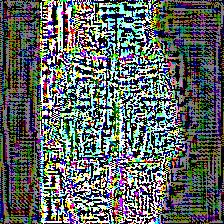
\includegraphics[width=3cm] {../thesis/images/adv/normal-24-epochs/fgsm/0.03/pertubation}};
\node [above=of pertubation, yshift=-1cm, color4, font=\small] {Pertubation};

\node [right=0.25cm of pertubation, inner sep=0.5pt, color3, font=\small] (equal) {$=$};

\node [rectangle, right=0.25cm of equal, inner sep=0.5pt, color3, draw, thick] (attack) {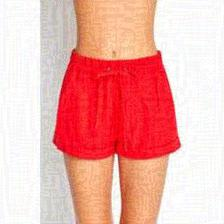
\includegraphics[width=3cm] {../thesis/images/adv/normal-24-epochs/fgsm/0.03/attack}};
\node [above=of attack, yshift=-1cm, color3, font=\small] {Adversarial};

\end{tikzpicture}
	\caption{Adversarial example, created using the \acs{FGSM} with $\epsilon = 0.03$. The perturbation is normalized for visualization purposes.}
	\label{fig:fgsm-example}
\end{figure}
The cosine distance of feature vectors before and after the attack for this example are:
\begin{align}
dist(\mathcal{F}(A),\,\mathcal{F}(T)) &= 0.6247 \\
dist(\mathcal{F}(A + \delta),\,\mathcal{F}(T)) &= 0.5267
\end{align}
Already from just looking at this one example, we can see that the achieved reduction in the cosine distance after the attack is quite limited and is not enough to achieve a significant rank within the nearest neighbors of the target article. As seen in Table~\ref{tab:fgsm-results}, this first impression is confirmed when we evaluate the success rates achieved by \ac{FGSM} on a broader set of attack tuples for $\epsilon$ values ranging from 0.01 to 0.05.
\begin{table}[H]
	\centering
	\begin{tabular}{ lccccc } 
		\toprule		
		& \multicolumn{5}{c}{Maximal Perturbation} \\
		\cmidrule{2-6}
		$rank_{min}$ & $\epsilon = 0.01$ & $\epsilon = 0.02$ & $\epsilon = 0.03$  & $\epsilon = 0.04$ & $\epsilon = 0.05$  \\
		\midrule
		1 & 0.12 & 0.07 & 0.06 & 0.02 & 0.01 \\
		3 & 0.27 & 0.16 & 0.14 & 0.09 & 0.07 \\
		10 & 0.64 & 0.44 & 0.32 & 0.18 & 0.13 \\
		100 & 2.87 & 2.45 & 1.83 & 1.36 & 0.99 \\
		\bottomrule
	\end{tabular}
	\caption{Success rates (\%) calculated over 10,000 random attack tuples using \acs{FGSM}.}
	\label{tab:fgsm-results}
\end{table}
The maximum success rate achieved using \ac{FGSM} for $rank_{min}=3$ in our experiments is 0.27\%, indicating that the one-step optimization step is not sufficient for successfully finding worst-case perturbations  that fulfill our adversary objective. The fact that the performance decreases with larger step sizes (higher $\epsilon$ values) reinforces this hypothesis.

To further illustrate the effect that our evaluated attacks have on the cosine distances of attack tuples, we introduce a scatter plot with a fitted quantile regression of the cosine distances before and after each attack. This plot can help us better understand the strengths and weaknesses of our attacks and defenses. For a perfectly robust model, all points should be located on this plot's identity (green dashed line). On the other hand, a perfect attack should be able to push all points toward the x-axis of this plot, minimizing the distances of all attack tuples to values very close to 0.0. 
\begin{figure}[H]
	\centering
	% This file was created by tikzplotlib v0.9.3.
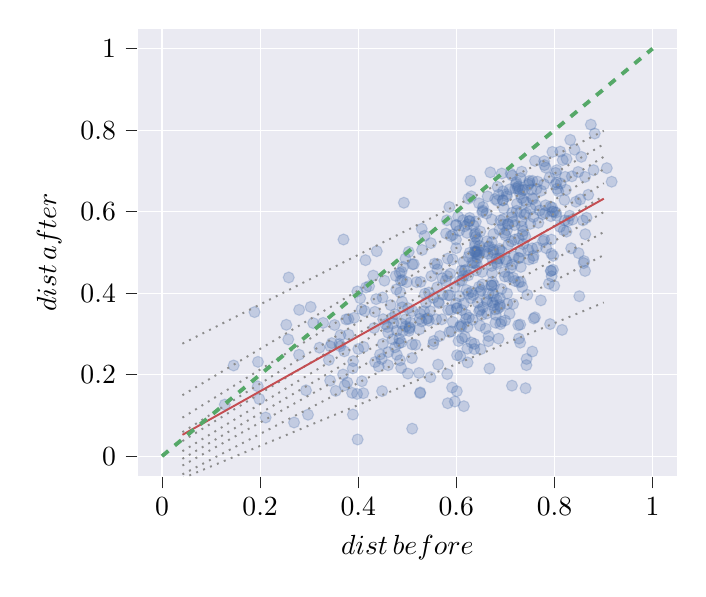
\begin{tikzpicture}

\definecolor{color0}{rgb}{0.917647058823529,0.917647058823529,0.949019607843137}
\definecolor{color1}{rgb}{0.298039215686275,0.447058823529412,0.690196078431373}
\definecolor{color2}{rgb}{0.768627450980392,0.305882352941176,0.32156862745098}
\definecolor{color3}{rgb}{0.333333333333333,0.658823529411765,0.407843137254902}

\begin{axis}[
axis background/.style={fill=color0},
axis line style={white},
tick align=outside,
tick pos=left,
x grid style={white},
xlabel={$dist\,before$},
xmajorgrids,
xmin=-0.05, xmax=1.05,
xtick style={color=white!15!black},
y grid style={white},
ylabel={$dist\,after$},
ymajorgrids,
ymin=-0.05, ymax=1.05,
ytick style={color=white!15!black}
]
\addplot [only marks, mark=*, draw=color1, fill=color1, opacity=0.25, colormap/blackwhite, clip marker paths=true]
table{%
	x                      y
	0.702415708370348 0.642774154303009
	0.754562265719132 0.509989611148213
	0.622942623777741 0.3169858349299
	0.703458344759386 0.398961772198442
	0.688668121265348 0.387834934386291
	0.675262502154267 0.500632098929902
	0.648764952983917 0.551304897355616
	0.715783589796988 0.373506515890916
	0.493125563624055 0.621771094408737
	0.694814559171798 0.628052882019278
	0.671926924051165 0.466847926530393
	0.610279462227697 0.45537775547314
	0.676768541955742 0.419641766920284
	0.682046829010273 0.484083204470962
	0.460768428064135 0.223191907679584
	0.682171316685205 0.383980895362687
	0.547159623836593 0.193881880595816
	0.483211624992775 0.276838071714836
	0.703973728075216 0.373857034676621
	0.536092193653216 0.398708862980787
	0.430563846575864 0.443050055244718
	0.793765993203607 0.531346282947941
	0.733123091593928 0.633375192502556
	0.375306138683051 0.335621160258593
	0.606871381929733 0.429680476599045
	0.713849065351361 0.688479022608963
	0.461173697046271 0.302770657932516
	0.601110597603032 0.362443902687503
	0.862311008104433 0.68521724291658
	0.198395032717312 0.140214790982265
	0.720342576671122 0.657307674046671
	0.8048166617147 0.701813490759316
	0.618347389902225 0.456827543318882
	0.589807353350653 0.306232153435818
	0.760260452188501 0.340621476636035
	0.475337249944287 0.348062800178635
	0.599374426244572 0.375229879585763
	0.538095642252625 0.376579578155321
	0.906715722327912 0.706770987860634
	0.499178475264685 0.427071752280542
	0.643581152267228 0.37667024252052
	0.691905609507933 0.410132751628219
	0.638159931200272 0.52361377327888
	0.476485971097163 0.44241452225928
	0.87421183191743 0.81345520543129
	0.639556209349192 0.50072495334102
	0.778680114406915 0.667270921946843
	0.725095818740654 0.656992638858032
	0.2574245180233 0.286447302918991
	0.60139832995532 0.247758981362113
	0.496895517332662 0.33620043188529
	0.700223625388336 0.541841852028288
	0.45544101855962 0.323573521627776
	0.726081080386389 0.661794900820584
	0.597019017771369 0.134045569360919
	0.623010220852823 0.229898923404874
	0.638318094472469 0.474650626131329
	0.552930358347523 0.274918823757852
	0.728956516410697 0.653585243425401
	0.592664367498009 0.543105718677939
	0.509380537490764 0.240611542200171
	0.562849608183515 0.224696152058779
	0.641843175966948 0.501561623322486
	0.762155444520558 0.616044019835303
	0.726821621582459 0.534226685547962
	0.742518828852618 0.622558991379304
	0.733225396639012 0.698065448966649
	0.52394088150878 0.204165854377893
	0.636711540835436 0.26278724923203
	0.722965177889884 0.602022262674786
	0.397642180223811 0.152632363690749
	0.665159140450771 0.282040637118135
	0.2793752505611 0.248838421401291
	0.780922728141505 0.596744498714598
	0.671464626390785 0.418646721614713
	0.75484078585268 0.256736481659546
	0.631294078928079 0.403121453327598
	0.502885803409256 0.501219106265865
	0.683971790582244 0.660794767787874
	0.582929843542721 0.395035347143723
	0.69774443094326 0.452022177642277
	0.746549052461539 0.506200505656518
	0.684260370882287 0.361584174263713
	0.47188236732971 0.326328747939585
	0.765551680172992 0.673659805314484
	0.648268205282123 0.32001652993907
	0.42222211309167 0.41701352235936
	0.354145695207815 0.16006300283864
	0.55386301946419 0.282521144528043
	0.588955962660916 0.358428996468041
	0.68611052593687 0.288368493520258
	0.797524070588607 0.491516742935771
	0.548145050195444 0.522667833519184
	0.346150736629563 0.277428328454829
	0.468889537369437 0.339106246605638
	0.680093259437724 0.346870648861539
	0.601365821114525 0.363446343030391
	0.728453220381975 0.486116341599983
	0.487725685303846 0.278987621587945
	0.570356366452542 0.335714608728282
	0.675510178612058 0.506135262197869
	0.586384882349238 0.394470445924202
	0.45992517400911 0.316810435081794
	0.188675375908656 0.353526398362496
	0.506634973765494 0.327747019188454
	0.582442181916682 0.12984747577223
	0.578130560821556 0.430424698709555
	0.450761328544105 0.336018668733389
	0.756453470620315 0.630661159820232
	0.794275094365343 0.441341674843165
	0.524743094571951 0.311311125926138
	0.79254369581027 0.58887302206539
	0.407498609875649 0.183827145911068
	0.449644392239964 0.389328216557515
	0.85472592271468 0.734364619861298
	0.804283800750059 0.589653937909185
	0.673922464001452 0.37651606959058
	0.667523793495931 0.215097182696438
	0.496268453287522 0.484705981253767
	0.483853353618334 0.287792924165156
	0.663804058997662 0.63732957029207
	0.411049132249338 0.267964629222522
	0.649516446813257 0.262448569248622
	0.692633702812703 0.693561248016207
	0.676696679592519 0.392099754548858
	0.647103966803853 0.500156725765981
	0.647085111785833 0.515901930718088
	0.848247121140365 0.697425919060439
	0.827408879963434 0.576807012437548
	0.832232486973633 0.776111993072592
	0.269253470095384 0.0825764715410656
	0.604482795390865 0.282428935621894
	0.760377548108937 0.724484179742531
	0.559082214374 0.335761943302
	0.571655158160587 0.436460076047361
	0.488854295748811 0.324597699265724
	0.44867509448027 0.159625831143221
	0.772711693358847 0.651264317923255
	0.475101836231654 0.266993515769663
	0.363466633524566 0.269874507442504
	0.783100949852193 0.510484310675257
	0.535179046372097 0.540560483804613
	0.737464498407575 0.627135057528081
	0.55581570611203 0.472345334108886
	0.437818409062504 0.502954381356507
	0.581462216039879 0.201224296268434
	0.389197207718035 0.10214034982045
	0.663981195622257 0.496812568357871
	0.748224351972533 0.482445898384373
	0.852641545401891 0.630053433146038
	0.488168880102405 0.452242412492601
	0.713832283231705 0.470112784023137
	0.662207354854433 0.527042121829788
	0.541792114147927 0.338371886654983
	0.727142595074989 0.426835495345802
	0.398808397490077 0.0409384198806303
	0.702779942377171 0.477969059788949
	0.41478878918773 0.480915193329852
	0.622873675599749 0.568705105915549
	0.776614676785678 0.52793709730069
	0.87980133940749 0.701801571088992
	0.32850483983967 0.327024573344363
	0.371631131105478 0.257214030367173
	0.510699230387221 0.356076187668874
	0.834164451252723 0.509954875054763
	0.754762385600963 0.632772462654478
	0.840964912351994 0.751926699219924
	0.391667277294795 0.339563973390972
	0.757330790874097 0.491617248389368
	0.726607872220438 0.486249827860925
	0.682473453499696 0.475509783632371
	0.748791159551174 0.675362791804116
	0.624439138406034 0.398859585594415
	0.665574481382659 0.398777877306244
	0.629651081971958 0.387805627871516
	0.70306252794346 0.637673426494287
	0.308363101673191 0.326435295988812
	0.484561674323491 0.44909253667475
	0.795185617162357 0.609904768635404
	0.211346263849501 0.0948246264112706
	0.342767533971448 0.18538268002243
	0.831005373704125 0.589887065823582
	0.791749108727719 0.612205901698674
	0.525489224871834 0.337347170655538
	0.626016797728373 0.576482105869948
	0.47020835761578 0.286868304749978
	0.734367248318005 0.41494671815105
	0.415933199389261 0.413876451229186
	0.639752268493246 0.575513225444319
	0.146054066915494 0.222502669523032
	0.434403747066271 0.231026804127679
	0.836832598446115 0.580546661092212
	0.195671484123418 0.231379800761953
	0.721535730803845 0.668225750711006
	0.487481876330227 0.216525505716494
	0.592411542529416 0.482839009114991
	0.616992206881338 0.564052063937713
	0.820778841759098 0.578409489440618
	0.638012050104955 0.516348660646185
	0.616337518455307 0.455154388852537
	0.581930990105471 0.441845329940247
	0.485172927600114 0.23529120503914
	0.675524866423059 0.545006383536312
	0.741148120821931 0.166660199955432
	0.687758507885261 0.485237792551661
	0.478698834255737 0.248938383815142
	0.72259414358091 0.672206569874941
	0.632305450729741 0.474865682589956
	0.65169690681596 0.346145726074336
	0.619984371056485 0.347387720459362
	0.673074063823612 0.427715451525898
	0.683197178202351 0.626859390583078
	0.81559063709552 0.309808333065398
	0.710700073977183 0.693364105633453
	0.713422554289352 0.173033803046335
	0.730170075637383 0.278424334194456
	0.767245143314486 0.57259374209347
	0.303068589918604 0.366228947069496
	0.63942643527706 0.547571557031388
	0.700478669182726 0.482918580811922
	0.733549840148094 0.56403236718016
	0.561154069688357 0.471388010333532
	0.585775163600264 0.611385423482342
	0.529462849479106 0.557779988436945
	0.61094518458691 0.358574579359857
	0.756445972009393 0.485214662101497
	0.703221588766225 0.554285284174179
	0.599928313334862 0.567770347375633
	0.862417595368404 0.45434417684936
	0.516686685497664 0.273319559841409
	0.585905409712199 0.3045201241405
	0.59969323140267 0.510399614480807
	0.67841678077485 0.360190421792543
	0.599815000756822 0.566195047409011
	0.363795197406286 0.296939204641106
	0.795826560427081 0.600013534865866
	0.859612729117633 0.473648746205306
	0.377849059904142 0.180784733141555
	0.641717334164208 0.496202931132122
	0.613820864913976 0.578947776886291
	0.705899724923756 0.570025490603023
	0.398223848644032 0.404231614486014
	0.779035190896361 0.723623959296325
	0.695298467793741 0.649996683367771
	0.404050096226184 0.387556415867583
	0.510471176576365 0.470692073039316
	0.636759969811764 0.275532223857032
	0.816861201373893 0.726521510591061
	0.73506814716465 0.543566967177009
	0.736206070385436 0.552251255221071
	0.478679264453424 0.307695611009567
	0.643004603379794 0.505535225920553
	0.453453782841143 0.430599344356504
	0.52604322513318 0.15448734363316
	0.293557438970808 0.161603044715851
	0.742502442226955 0.595727619294325
	0.549017575820898 0.441851385310269
	0.340198714796918 0.23611860919523
	0.432407148633786 0.314584889056385
	0.638147665980114 0.501690668821203
	0.862867265520115 0.544645026179943
	0.793241934930854 0.455124356655304
	0.617450678241407 0.292891104168866
	0.80785991708086 0.650293158721395
	0.504537545577303 0.316333660412681
	0.406820546876471 0.360342649142435
	0.694959933188981 0.627387965019454
	0.818900513117869 0.554219236561925
	0.843768630019062 0.624230233622789
	0.447757459088158 0.238483322676517
	0.77949671027167 0.714265564626827
	0.735997737840423 0.520305662199331
	0.633015735275752 0.334570425594646
	0.726318793272189 0.321456983290492
	0.637385874853177 0.544547695718407
	0.620778042805058 0.407606893829046
	0.705983005502186 0.519566834897622
	0.779442813901686 0.531323233598751
	0.503370964168937 0.307391877703067
	0.811941509864712 0.74725456272843
	0.351827817907211 0.321875448883503
	0.688927447590167 0.366243748141429
	0.641805529774103 0.470477069077866
	0.624449096924229 0.631893851929308
	0.627295479219605 0.499111470308418
	0.757106866080272 0.587178801508735
	0.740464606727979 0.538853828403329
	0.6531029663179 0.421395929145446
	0.63725820331713 0.501771575643673
	0.683185028644089 0.471808010929743
	0.717199570098645 0.489669883949874
	0.799587565912047 0.418002062242316
	0.501735933870344 0.363081895498024
	0.803073308580441 0.597733998410104
	0.672866768880645 0.486353432979512
	0.789975778535569 0.683186586542181
	0.592798446198032 0.329287328193457
	0.477742486518353 0.409268896795631
	0.71260933919927 0.586514998445171
	0.751759781331414 0.606576161710143
	0.719437092843027 0.429873837747141
	0.708592909016867 0.654621350422551
	0.812591198659877 0.669081051328651
	0.82471400668633 0.729310250069916
	0.489901831213194 0.432035845349632
	0.648287290988695 0.403491294198962
	0.596710301408254 0.415653132681678
	0.671713560988895 0.418894783860221
	0.627107320647832 0.577515531752317
	0.730778957405236 0.682159217248909
	0.433940428717105 0.354213038373505
	0.627190435073763 0.5845488552673
	0.566527958409685 0.29481008558187
	0.625694597140793 0.33990114610478
	0.543964031023018 0.40148588670593
	0.611496515446837 0.431738161160579
	0.672287030833304 0.580753634623901
	0.795769438681675 0.746506463157405
	0.546568133215569 0.355946094751661
	0.588715107762576 0.540178179990452
	0.821911985900082 0.685265801781774
	0.279621508310043 0.359031867451706
	0.85812332157074 0.578465947585667
	0.624759536462276 0.489352209678143
	0.71606123020989 0.575431512351802
	0.797122328636563 0.45732057737149
	0.654407494616176 0.611381162910838
	0.489854397730834 0.365191222932238
	0.860402619940149 0.478764132617508
	0.662445043507389 0.350181043285082
	0.802320255845057 0.695057237255472
	0.865475085063675 0.584911128027787
	0.525982870293736 0.349602964923364
	0.491697839328053 0.464462889380214
	0.369203803880366 0.200432205336844
	0.688025098290681 0.508785674389386
	0.63537522120738 0.473704888583488
	0.750894843204854 0.570045286969876
	0.526512605089327 0.15644650005327
	0.715935513921598 0.437775145774692
	0.729845643297626 0.643416206672637
	0.690022712222139 0.578787215582392
	0.698041580334336 0.547329151262469
	0.667302734936837 0.514436495005286
	0.607033556282618 0.317613323373315
	0.621731245740836 0.547968753143665
	0.772259934556409 0.382261375247639
	0.489265183880399 0.379053994003665
	0.389720848513221 0.233124537833726
	0.688054658794603 0.555680560096827
	0.672253291965108 0.525437452786672
	0.53012883991183 0.505953155696455
	0.572258243892152 0.396102094329223
	0.66252997059314 0.378161140149057
	0.804437219741749 0.671380801910917
	0.461338712073134 0.255242050821469
	0.534306471568606 0.355642653793039
	0.6968890826198 0.607762873189903
	0.732806164479613 0.577300734609963
	0.746845496754968 0.666239227901737
	0.321145534629901 0.266146983835297
	0.643139394196085 0.486663519404383
	0.672992234181883 0.449265359352692
	0.297658885232463 0.101744185687143
	0.68626076969798 0.641408837205194
	0.380512884184121 0.298173455773324
	0.91658672056603 0.673389185993012
	0.665782027061534 0.294739732303917
	0.752603466680578 0.654311606305878
	0.661265692066871 0.383318774804887
	0.748721617134568 0.670182705644529
	0.659711290784149 0.312909753201889
	0.78208511095306 0.615502062429621
	0.658128918898406 0.501878166416327
	0.74473391028788 0.395847611727472
	0.723569269956923 0.619054213796458
	0.78879209727135 0.423305209199315
	0.628736329889625 0.675687705872156
	0.564493479078452 0.3756727684227
	0.674686481616019 0.400109322838059
	0.664902503258122 0.512777205475817
	0.849238073295175 0.498136400720811
	0.501228304990483 0.202624632960361
	0.882133776905331 0.79163730027802
	0.630528709798755 0.278836019528569
	0.70647706238952 0.439616096467416
	0.71363838206889 0.597179367419802
	0.646365786538809 0.415653349225586
	0.688900721215907 0.370821814311536
	0.619682018076226 0.336230309494912
	0.718922944722599 0.566993140422997
	0.811184798347269 0.56269622195972
	0.687925186136757 0.504531741955559
	0.387552656858457 0.15540186357962
	0.372449531923922 0.173832801517958
	0.615314443652391 0.122575857494271
	0.582554436433109 0.484772017072825
	0.735649207981884 0.653053231316442
	0.679707310912721 0.327406255076018
	0.69486355463193 0.56821543372708
	0.583328471482801 0.359130373201435
	0.466180003250447 0.370723025099313
	0.776358377570657 0.593615165590564
	0.258360552567522 0.438412643650084
	0.801974858427969 0.666843716482336
	0.648179401054582 0.359365405958585
	0.639159820692509 0.538176576623138
	0.529141750475455 0.330656823915145
	0.730283461359713 0.322807596182226
	0.614841970351346 0.476633831142485
	0.504509585098985 0.312992968875189
	0.591335811027096 0.16843767527702
	0.712049368186565 0.526981164086723
	0.513241827912513 0.471272518182221
	0.731393786601958 0.464369514065632
	0.652500007880352 0.45204268203632
	0.676786992234083 0.370473582044267
	0.645926140726445 0.4943965785725
	0.738583752673319 0.592905194134199
	0.5614618340096 0.458263113645113
	0.652944273746731 0.599231413582463
	0.646210028606477 0.620406941325193
	0.606566065037108 0.3922643868981
	0.689664402402135 0.324026660551012
	0.642981963042991 0.532278646408502
	0.361879435980638 0.275098797817366
	0.743221891158461 0.238512459204288
	0.538739747307561 0.336273073443395
	0.708557745621835 0.349239711096634
	0.692821381049714 0.502225012100076
	0.850663757271779 0.392436209693918
	0.661287078756062 0.59541768361534
	0.56097878592788 0.414423482977496
	0.553060828726945 0.388658668085669
	0.490862629336511 0.306665707324177
	0.7578495940198 0.33775522219258
	0.718606464389788 0.531365893495663
	0.624237073648552 0.443515344530799
	0.692107357695437 0.329736695639762
	0.769947772371584 0.602856324875455
	0.71124619359563 0.462340147413913
	0.755240762949048 0.675457955810144
	0.370026388231088 0.531609729201014
	0.793643920084901 0.496814086350872
	0.646472271731773 0.35566502884135
	0.61117440018875 0.318336928707641
	0.608220117180946 0.245422025730228
	0.343310269317154 0.269307875683737
	0.450047657081826 0.275404794069165
	0.699361903234712 0.332937054280073
	0.253435352605208 0.322360394720796
	0.127993003301146 0.126511058531582
	0.731097758733111 0.427708936825046
	0.380123112784097 0.336439512247898
	0.868830487902042 0.641262462623449
	0.704877108097704 0.568856844800757
	0.543896631801827 0.332461138876374
	0.731478532497142 0.502078644603655
	0.195232315580379 0.171433712249534
	0.599450494650076 0.531587220876224
	0.563455440316046 0.378775177342115
	0.696004075507836 0.581217843902317
	0.615226778166779 0.374337397170652
	0.410476630123713 0.154467381670789
	0.587527433522299 0.447633606553931
	0.630406725281677 0.637594808954609
	0.791024122954258 0.324094469288885
	0.730636183940409 0.598710143537154
	0.679151783466294 0.630986674517021
	0.698919668402146 0.440844994614611
	0.742887204206143 0.223341502953674
	0.436566686896686 0.385389595276631
	0.609462456428024 0.32168464395084
	0.622355435787681 0.263784965304485
	0.764303039400215 0.511897366936349
	0.63433767076546 0.395040363111441
	0.444432521671225 0.249357084314234
	0.51006177433115 0.0674649855663626
	0.388781357206453 0.215572167225022
	0.605684220469654 0.552943110880294
	0.486660907182626 0.430648229682991
	0.654408934433279 0.365597332998428
	0.614899182429451 0.442673243776933
	0.835395492848672 0.686597234372636
	0.601056289327821 0.159430687156633
	0.509766855559688 0.274143530646002
	0.611445001469363 0.288904090705353
	0.579047581945019 0.546169754991945
	0.669324854551684 0.6963957155084
	0.792455183999777 0.454311398738114
	0.635229875845389 0.565815851147976
	0.400168617523983 0.262975506998653
	0.653890481451795 0.602359620769623
	0.782144367009361 0.707962481548889
	0.52727393912818 0.42767761194703
	0.580775670446844 0.578745616770201
	0.740365160570812 0.653646182423421
	0.640367290279946 0.455925823689385
	0.727548449439151 0.288481458390338
	0.805354252865787 0.655946063493213
	0.650360016883162 0.407086350421411
	0.485520007631953 0.402022147300494
	0.496825095166324 0.318528279738741
	0.441824899173361 0.219882998378248
	0.820383400035779 0.628533758093009
	0.519159056086118 0.427081808139506
	0.824520010570703 0.550852154521391
	0.763567168662914 0.656041935051976
	0.603539427984282 0.587952163555323
	0.413336885070322 0.356131905771098
	0.823316546553899 0.653580077755678
	0.798589604254776 0.599790448632219
};
\addplot [line width=0.7pt, white!54.9019607843137!black, dotted]
table {%
	0.0417168782132947 -0.0544346657920543
	0.137148593984546 -0.00650221572517698
	0.232580309755798 0.0414302343417003
	0.328012025527049 0.0893626844085776
	0.423443741298301 0.137295134475455
	0.518875457069553 0.185227584542332
	0.614307172840804 0.233160034609209
	0.709738888612056 0.281092484676087
	0.805170604383307 0.329024934742964
	0.900602320154559 0.376957384809841
};
\addplot [line width=0.7pt, white!54.9019607843137!black, dotted]
table {%
	0.0417168782132947 -0.0446753269267379
	0.137148593984546 0.0151158034543915
	0.232580309755798 0.0749069338355209
	0.328012025527049 0.13469806421665
	0.423443741298301 0.19448919459778
	0.518875457069553 0.254280324978909
	0.614307172840804 0.314071455360039
	0.709738888612056 0.373862585741168
	0.805170604383307 0.433653716122297
	0.900602320154559 0.493444846503427
};
\addplot [line width=0.7pt, white!54.9019607843137!black, dotted]
table {%
	0.0417168782132947 -0.0230406280969271
	0.137148593984546 0.0406265915342204
	0.232580309755798 0.104293811165368
	0.328012025527049 0.167961030796515
	0.423443741298301 0.231628250427663
	0.518875457069553 0.29529547005881
	0.614307172840804 0.358962689689958
	0.709738888612056 0.422629909321105
	0.805170604383307 0.486297128952253
	0.900602320154559 0.5499643485834
};
\addplot [line width=0.7pt, white!54.9019607843137!black, dotted]
table {%
	0.0417168782132947 -0.00653406749328027
	0.137148593984546 0.0607515617353202
	0.232580309755798 0.128037190963921
	0.328012025527049 0.195322820192521
	0.423443741298301 0.262608449421122
	0.518875457069553 0.329894078649722
	0.614307172840804 0.397179707878322
	0.709738888612056 0.464465337106923
	0.805170604383307 0.531750966335523
	0.900602320154559 0.599036595564124
};
\addplot [line width=0.7pt, white!54.9019607843137!black, dotted]
table {%
	0.0417168782132947 0.0122713460115122
	0.137148593984546 0.0818894520679209
	0.232580309755798 0.15150755812433
	0.328012025527049 0.221125664180738
	0.423443741298301 0.290743770237147
	0.518875457069553 0.360361876293555
	0.614307172840804 0.429979982349964
	0.709738888612056 0.499598088406373
	0.805170604383307 0.569216194462781
	0.900602320154559 0.63883430051919
};
\addplot [line width=0.7pt, white!54.9019607843137!black, dotted]
table {%
	0.0417168782132947 0.0370300204532863
	0.137148593984546 0.107311176788782
	0.232580309755798 0.177592333124277
	0.328012025527049 0.247873489459773
	0.423443741298301 0.318154645795269
	0.518875457069553 0.388435802130764
	0.614307172840804 0.45871695846626
	0.709738888612056 0.528998114801755
	0.805170604383307 0.599279271137251
	0.900602320154559 0.669560427472746
};
\addplot [line width=0.7pt, white!54.9019607843137!black, dotted]
table {%
	0.0417168782132947 0.0589562903223723
	0.137148593984546 0.130679359800868
	0.232580309755798 0.202402429279363
	0.328012025527049 0.274125498757859
	0.423443741298301 0.345848568236354
	0.518875457069553 0.417571637714849
	0.614307172840804 0.489294707193345
	0.709738888612056 0.56101777667184
	0.805170604383307 0.632740846150335
	0.900602320154559 0.704463915628831
};
\addplot [line width=0.7pt, white!54.9019607843137!black, dotted]
table {%
	0.0417168782132947 0.0945219582737153
	0.137148593984546 0.165650441789156
	0.232580309755798 0.236778925304596
	0.328012025527049 0.307907408820037
	0.423443741298301 0.379035892335477
	0.518875457069553 0.450164375850918
	0.614307172840804 0.521292859366359
	0.709738888612056 0.592421342881799
	0.805170604383307 0.66354982639724
	0.900602320154559 0.73467830991268
};
\addplot [line width=0.7pt, white!54.9019607843137!black, dotted]
table {%
	0.0417168782132947 0.149598153356871
	0.137148593984546 0.218046431163341
	0.232580309755798 0.28649470896981
	0.328012025527049 0.35494298677628
	0.423443741298301 0.42339126458275
	0.518875457069553 0.49183954238922
	0.614307172840804 0.560287820195689
	0.709738888612056 0.628736098002159
	0.805170604383307 0.697184375808629
	0.900602320154559 0.765632653615099
};
\addplot [line width=0.7pt, white!54.9019607843137!black, dotted]
table {%
	0.0417168782132947 0.276004466582372
	0.137148593984546 0.334030127650461
	0.232580309755798 0.39205578871855
	0.328012025527049 0.45008144978664
	0.423443741298301 0.508107110854729
	0.518875457069553 0.566132771922818
	0.614307172840804 0.624158432990907
	0.709738888612056 0.682184094058997
	0.805170604383307 0.740209755127086
	0.900602320154559 0.798235416195175
};
\addplot [line width=0.7pt, color2]
table {%
	0.0417168782132947 0.0523671042919516
	0.137148593984546 0.116749778174322
	0.232580309755798 0.181132452056693
	0.328012025527049 0.245515125939064
	0.423443741298301 0.309897799821435
	0.518875457069553 0.374280473703805
	0.614307172840804 0.438663147586176
	0.709738888612056 0.503045821468547
	0.805170604383307 0.567428495350917
	0.900602320154559 0.631811169233288
};
\addplot [line width=1.4pt, color3, dashed]
table {%
	0 0
	1 1
};
\end{axis}

\end{tikzpicture}

	\caption{Quantile regression plot of 512 sampled cosine distances between target and attack article, before and after performing \acs{FGSM} attacks, using $\epsilon=0.05$}
	\label{fig:fgsm-quantile}
\end{figure}
When attacking our undefended model using the \ac{FGSM} attack with $\epsilon=0.05$, we see a pretty mixed result in Figure~\ref{fig:fgsm-quantile}. While the attack reduced some distances, many other distances increased after the attack, indicating failed approximations of the actual loss surface. This plot confirms our previous findings, indicating that the \ac{FGSM} attack is unsuitable for our targeted adversary objective.

\subsection{Projected Gradient Descent}
For \acl{PGD} we use a step size of $\alpha=\frac{\epsilon}{k}$ where $k$ is the number of total iterations. In the following section, we assess the effectiveness of the iterative \acl{PGD} method using $k=(8, 16, 32, 64, 128)$ for optimizing our adversarial goal. An example attack tuple calculated using \ac{PGD} can be seen in Figure~\ref{fig:pgd-example}. 
\begin{figure}[H]
	\centering
	\begin{tikzpicture}
\node [rectangle, inner sep=0.5pt, color1, draw, thick] (target) {\includegraphics[width=3cm] {../thesis/images/adv/target}};
\node [above=of target, yshift=-1cm, color1, font=\small] {Target};

\node [rectangle, right=1cm of target, inner sep=0.5pt,color2, draw, thick] (original) {\includegraphics[width=3cm] {../thesis/images/adv/original}};
\node [above=of original, yshift=-1cm, color2, font=\small] {Original};

\node [right=0.25cm of original, inner sep=0.5pt, color4, font=\small] (plus) {$+$};

\node [rectangle, right=0.25cm of plus, inner sep=0.5pt, color4, draw, thick] (pertubation) {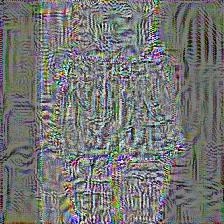
\includegraphics[width=3cm] {../thesis/images/adv/normal-24-epochs/pgd/0.03/pertubation}};
\node [above=of pertubation, yshift=-1cm, color4, font=\small] {Pertubation};

\node [right=0.25cm of pertubation, inner sep=0.5pt, color3, font=\small] (equal) {$=$};

\node [rectangle, right=0.25cm of equal, inner sep=0.5pt, color3, draw, thick] (attack) {\includegraphics[width=3cm] {../thesis/images/adv/normal-24-epochs/pgd/0.03/attack}};
\node [above=of attack, yshift=-1cm, color3, font=\small] {Adversarial};

\end{tikzpicture}
	\caption{Adversarial example, created using \acs{PGD} with $\epsilon = 0.03$ and $32$ iterations. The perturbation is normalized for visualization purposes.}
	\label{fig:pgd-example}
\end{figure}
The cosine distance of feature vectors before and after the attack for this example are:
\begin{align}
dist(\mathcal{F}(A),\,\mathcal{F}(T)) &= 0.6247 \\
dist(\mathcal{F}(A + \delta),\,\mathcal{F}(T))) &= 0.0500
\end{align}
Judging by this one example, we can already see that the achieved reduction in the cosine distance after the attack is significantly higher than in the case of \ac{FGSM} and is high enough to successfully rank on the first place among the nearest neighbors of the target article. The effect that a successful injection of this adversarial example into the product catalog would have on the resulting recommendations for the target article is shown in Figure~\ref{fig:pgd-reco}. As seen in Table~\ref{tab:pgd-results}, this first impression is confirmed once again when we evaluate the success rates achieved by \ac{PGD} with 64 iterations on a broader set of attack tuples for $\epsilon$ values ranging from 0.01 to 0.05.
\begin{figure}[H]
	\centering
	\begin{tikzpicture}


\node [rectangle, inner sep=0.5pt, color1, draw, thick] (query) {\includegraphics[width=3cm] {../thesis/images/adv/target}};
\node [above=of query, yshift=-1cm, color1, font=\small] {\textbf{Query} image};


\node [right=of query.north east, rectangle, inner sep=0.5pt, color2, draw, thick] (orig1) {\includegraphics[width=2cm] {../../data/DeepFashion/img_resized/Mixed_Media_Knit_Tee/img_00000046.jpg}};
\node [above=of orig1, yshift=-1cm, color2, font=\small] {$dist = 0.0596$};

\node [right=0.5cm of orig1, rectangle, inner sep=0.5pt, color2, draw, thick] (orig2) {\includegraphics[width=2cm] {../../data/DeepFashion/img_resized/Striped_Boat_neck_Tee/img_00000088.jpg}};
\node [above=of orig2, yshift=-1cm, color2, font=\small] {$dist = 0.0615$};

\node [right=0.5cm of orig2, rectangle, inner sep=0.5pt, color2, draw, thick] (orig3) {\includegraphics[width=2cm] {../../data/DeepFashion/img_resized/Boat_Neck_Striped_Top/img_00000013.jpg}};
\node [above=of orig3, yshift=-1cm, color2, font=\small] {$dist = 0.0656$};

\node [right=0.5cm of orig3, rectangle, inner sep=0.5pt, color2, draw, thick] (orig4) {\includegraphics[width=2cm] {../../data/DeepFashion/img_resized/Nautical-Striped_Cotton_Tee/img_00000042.jpg}};
\node [above=of orig4, yshift=-1cm, color2, font=\small] {$dist = 0.0660$};


\node [right=of query.south east, rectangle, inner sep=0.5pt, color3, draw, thick] (adv1) {\includegraphics[width=2cm] {../thesis/images/adv/normal-24-epochs/pgd/0.03/attack}};
\node [above=of adv1, yshift=-1cm, color3, font=\small] {$dist = 0.0500$};

\node [right=0.5cm of adv1, rectangle, inner sep=0.5pt, color3, draw, thick] (adv2) {\includegraphics[width=2cm] {../../data/DeepFashion/img_resized/Mixed_Media_Knit_Tee/img_00000046.jpg}};
\node [above=of adv2, yshift=-1cm, color3, font=\small] {$dist = 0.0596$};

\node [right=0.5cm of adv2, rectangle, inner sep=0.5pt, color3, draw, thick] (adv3) {\includegraphics[width=2cm] {../../data/DeepFashion/img_resized/Striped_Boat_neck_Tee/img_00000088.jpg}};
\node [above=of adv3, yshift=-1cm, color3, font=\small] {$dist = 0.0615$};

\node [right=0.5cm of adv3, rectangle, inner sep=0.5pt, color3, draw, thick] (adv4) {\includegraphics[width=2cm] {../../data/DeepFashion/img_resized/Boat_Neck_Striped_Top/img_00000013.jpg}};
\node [above=of adv4, yshift=-1cm, color3, font=\small] {$dist = 0.0656$};


\end{tikzpicture}
	\caption{Ranked recommendation results for original \acs{k-NN} index (top) and manipulated index with injected \acs{PGD} adversarial example (bottom)}
	\label{fig:pgd-reco}
\end{figure}
\begin{table}[H]
	\centering
	\begin{tabular}{ lccccc } 
		\toprule		
		& \multicolumn{5}{c}{Maximal Perturbation} \\
		\cmidrule{2-6}
		$rank_{min}$ & $\epsilon = 0.01$ & $\epsilon = 0.02$ & $\epsilon = 0.03$  & $\epsilon = 0.04$ & $\epsilon = 0.05$  \\
		\midrule
		1 & 36.44 & 77.81 & 86.81 & 89.65 & 91.02 \\
		3 & 44.33 & 86.40 & 94.06 & 96.13 & 97.09 \\
		10 & 50.21 & 89.61 & 95.90 & 97.56 & 98.22 \\
		100 & 62.55 & 94.13 & 97.95 & 98.74 & 99.13 \\
		\bottomrule
	\end{tabular}
	\caption{Success rates (\%) calculated over 10,000 random attack tuples using \acs{PGD}-64.}
	\label{tab:pgd-results}
\end{table}
The maximum success rate for $rank_{min}=3$ achieved using \ac{PGD} with 64 iterations in our experiments is 97.09\%, indicating that an iterative optimization approach, like \ac{PGD}, is significantly more effective at successfully finding worst-case perturbations that fulfill our adversary objective. These results are consistent with the scientific consensus that iterative optimization-based attacks are strictly stronger than single-step attacks and should achieve strictly superior performance in a white-box setting \parencite{athalye2018obfuscated}. When we look at the impact on the cosine distances in Figure~\ref{fig:pgd-quantile}, we see a drastic improvement compared to \ac{FGSM}. Almost all points were successfully pushed onto the x-axis. Nonetheless, there is still room for improvement, as the spread of points with higher initial distances increases significantly.
\begin{figure}[H]
	\centering
	% This file was created by tikzplotlib v0.9.3.
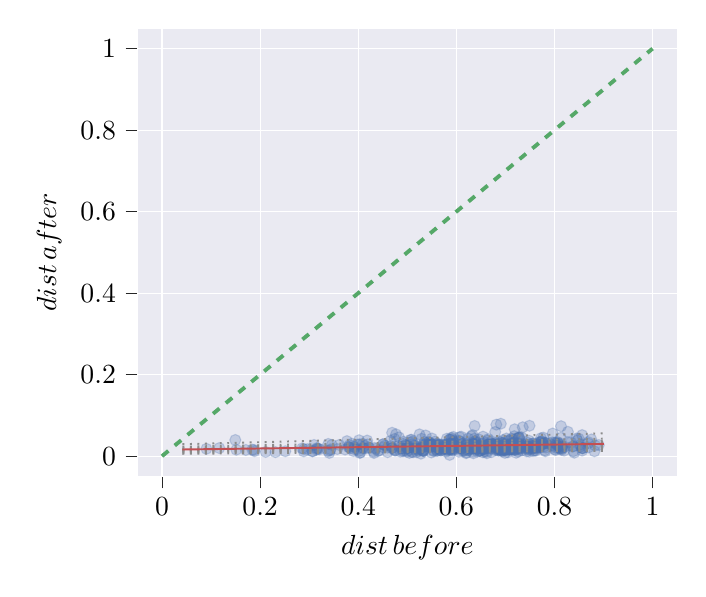
\begin{tikzpicture}

\definecolor{color0}{rgb}{0.917647058823529,0.917647058823529,0.949019607843137}
\definecolor{color1}{rgb}{0.298039215686275,0.447058823529412,0.690196078431373}
\definecolor{color2}{rgb}{0.768627450980392,0.305882352941176,0.32156862745098}
\definecolor{color3}{rgb}{0.333333333333333,0.658823529411765,0.407843137254902}

\begin{axis}[
axis background/.style={fill=color0},
axis line style={white},
tick align=outside,
tick pos=left,
x grid style={white},
xlabel={$dist\,before$},
xmajorgrids,
xmin=-0.05, xmax=1.05,
xtick style={color=white!15!black},
y grid style={white},
ylabel={$dist\,after$},
ymajorgrids,
ymin=-0.05, ymax=1.05,
ytick style={color=white!15!black}
]
\addplot [only marks, mark=*, draw=color1, fill=color1, opacity=0.25, colormap/blackwhite, clip marker paths=true]
table{%
x                      y
0.696670161927995 0.0321100780243553
0.846575950495874 0.0386062367753204
0.697437751763024 0.0145484704291969
0.251398122690762 0.0119769544629127
0.315056542097085 0.0194114767825164
0.689078359479143 0.0148986408150824
0.663981195622257 0.0386871722083656
0.589875808578639 0.0450648040680781
0.673286087753526 0.0291266719901438
0.433124409038849 0.0202317423708193
0.730026154401056 0.0233150078817561
0.561484527820804 0.0133692533993033
0.719186578714695 0.0155713911690455
0.709165278702433 0.0167145598668219
0.661141332008263 0.0257999129257825
0.7260778529752 0.0193788074168068
0.812882125879595 0.0448015861768484
0.744817860750536 0.0220603126987871
0.499134637462377 0.0111378221849805
0.756922376070044 0.0255975093714093
0.719688614925708 0.0169654352463013
0.623325470160647 0.0144704265136368
0.637074900692242 0.043164267079751
0.603511445901255 0.021476918035209
0.636347628226877 0.0358029860249459
0.595362785120506 0.0169304382929881
0.868949257356209 0.0346464902730018
0.652265923486484 0.0164917575992671
0.705523438618546 0.0366921710249078
0.733671799507987 0.0139575324702024
0.569822086373427 0.018214902253319
0.531678345125916 0.014173705381054
0.403061363219696 0.00801486939759299
0.626323184727909 0.0189208551808524
0.52953507124363 0.0212255685493785
0.416280525770858 0.019162128969229
0.481462509107996 0.0252862176678483
0.632745521528226 0.0294894444811292
0.71840354189909 0.0240041485142963
0.772599138305656 0.044176962707995
0.725312897915575 0.0440261816684614
0.875252933072882 0.0410268422245434
0.418239281751631 0.0383381418457738
0.711462044711746 0.0294822813642792
0.387135803962687 0.030638368486541
0.761749033019123 0.0194870263007835
0.780331260907567 0.0145396774897427
0.506372111452881 0.0399998283331259
0.500345977417786 0.025892982781002
0.549018905892908 0.00903167337661936
0.413657683023549 0.0253239034745861
0.63063348473482 0.0486383591936284
0.633222178251343 0.0518143299921813
0.769679113913174 0.0343792770325994
0.17098995055103 0.0151831405997402
0.68122517785798 0.0147096515166987
0.285767107026719 0.0191932072095885
0.513841968873202 0.0262073512948153
0.532542008233391 0.0288430643383825
0.591350080939088 0.0418607474557731
0.688844595858073 0.0346075259677134
0.707956475578405 0.0194218660374049
0.544205270783398 0.0349939841843417
0.643088572473028 0.0113726108525365
0.802585330946842 0.0149339608739231
0.765596199364631 0.029660020116869
0.626870772721323 0.0245730997293592
0.511998167260823 0.00952596671763839
0.697745342193583 0.0153885362080388
0.605081813791851 0.038086381903457
0.66121495233487 0.0195785259770489
0.546542409137623 0.0310731656931906
0.695043871925535 0.0169169445956444
0.751116886492982 0.0183844086482741
0.698892975265683 0.0191632925558406
0.70080289487395 0.0243910158991243
0.675297661130235 0.0279829825223277
0.57743060842463 0.0256456177567799
0.491137329341159 0.0119264637500783
0.78292040323452 0.0314942355556541
0.716753856687077 0.0284108354090379
0.581850740679645 0.0258459624349129
0.639556209349192 0.0262571605833174
0.694254015522779 0.0214595961326297
0.450685176935258 0.0218523582075304
0.620627193103124 0.0264109150351318
0.540107973935503 0.0329631359148168
0.717363433208236 0.0343293312440687
0.696129125290798 0.0281836131050541
0.701439233853926 0.019134853162969
0.533079760967769 0.0132155748488857
0.404273872041391 0.00870439564504399
0.743221891158461 0.0117426738750201
0.662613420319498 0.0289662906464726
0.628201980641292 0.0273963925584533
0.553856580916107 0.0123079267277346
0.853461358666213 0.0236316744600945
0.679292072447462 0.0593900947187245
0.685663545285529 0.0177945819063897
0.815981952926438 0.0186611140169445
0.546613779479263 0.0275851085832118
0.720711175891001 0.0152882589833485
0.746681953130193 0.032714701222727
0.606457382672503 0.0465521859651189
0.469074304810784 0.0574110727075325
0.346198849244352 0.0275889320995312
0.466180003250447 0.0247749681039828
0.798606072188635 0.0247311427671798
0.671071681251416 0.0181540286560761
0.83378372506429 0.0339002331316081
0.80131722446853 0.0337343010578764
0.662318893955092 0.00717325780490141
0.658991065055317 0.0181346262010427
0.634794703159155 0.00710263790647925
0.693566091357552 0.0186383819699271
0.64535775017173 0.0415652995665953
0.640002131174986 0.0182034165224987
0.692790629885459 0.032329102587666
0.70056416962077 0.0157560205102159
0.47414931304442 0.0421316736049844
0.342454887341734 0.0139937511885242
0.553059553125412 0.0250248609063159
0.795763624986851 0.0338102680974366
0.361199438108516 0.0275025888284633
0.373296857827248 0.0161824927211313
0.477172639816737 0.0536576631720515
0.687227999042908 0.0210186417266025
0.670602879004158 0.0340865162832724
0.856487134873756 0.0517344198164797
0.316587325678127 0.0189548850433414
0.338967790249104 0.0300887396205053
0.70213782448763 0.0433818890773484
0.492259706624414 0.0353056545240304
0.546137019366367 0.031887305988458
0.654407494616176 0.0479067503150059
0.650532675948289 0.0216618401817584
0.868804760890495 0.0312195553284556
0.62070297191227 0.0090234706382023
0.675599484510648 0.0255899664137016
0.288869298503126 0.0117786809098736
0.547045382790052 0.0213058912571713
0.692903821782505 0.0219717931170446
0.808171122814947 0.0303631332452738
0.560049668181612 0.0208349753158815
0.55592112562195 0.0355050243662314
0.770971685186555 0.0342554435645719
0.613896248572504 0.0122678873598094
0.698241918326098 0.0281193971378199
0.6542660577321 0.0309791513921525
0.459895145615028 0.0207704356236517
0.718247221725794 0.0490800325847104
0.692218610961585 0.0192856893107174
0.663744649199595 0.0215185363896823
0.532336785507586 0.0155380402332352
0.774524343922366 0.0352667275040758
0.776630237688848 0.0311990087373668
0.660085494748534 0.0215039875865283
0.588715107762576 0.0313441774704093
0.624553744747329 0.0154550868471902
0.717484061862175 0.0209812162038914
0.526044716423777 0.0188381412839341
0.715763895989028 0.0200878502258408
0.773409262620881 0.0362711613147569
0.734063505786257 0.0243391734793473
0.778188619018219 0.0232031951257708
0.451120281543283 0.0293593405962179
0.584966543531128 0.0178093512156106
0.693585410450086 0.0229763905631897
0.690305109445003 0.0346590757316499
0.853775824745605 0.0286233129170562
0.607731458945772 0.0223024971158925
0.519200942772004 0.00962105134817803
0.759650442139145 0.0139288847545249
0.685808072088178 0.0130888827022181
0.63751176356306 0.0279148897413143
0.595686281446961 0.0218823168570883
0.496351955498791 0.0270776342846499
0.767911411547415 0.0216390388109752
0.63275069051416 0.0245994576162027
0.594492769416936 0.0268172010392481
0.66529090480384 0.041956564022492
0.549534657592614 0.028829100930277
0.65017608464948 0.0139681074154434
0.637679510255976 0.0290921924733565
0.528342730198252 0.0242256495620956
0.184244321846186 0.0158914336177512
0.636217108815598 0.0281883471002534
0.588866616457055 0.0170024540714725
0.623981833132033 0.0433587012765653
0.485938274971863 0.0110946678538737
0.641171019268431 0.0330782994204821
0.440378689971238 0.0125620459828202
0.383718105167242 0.0194431250214783
0.726825451696961 0.0458767330915395
0.654048372043022 0.00936277713309719
0.296344216541784 0.0171931352530541
0.432182139442709 0.00779143456769227
0.586892649068286 0.029160297389594
0.690624358682331 0.0795971765901835
0.674355945540299 0.0241528146327085
0.638452859640143 0.020753522684913
0.490862629336511 0.018988325095857
0.699037115104042 0.0271312439359203
0.321145534629901 0.0168646296007273
0.533333052028919 0.0226059117006435
0.535556359768757 0.0261706043529946
0.614038086870692 0.0316264198755937
0.639484465227291 0.0365324986177233
0.0906084946588799 0.0179845924074771
0.781845355838316 0.0317236868526724
0.857710040160883 0.0189786854946913
0.795064376353096 0.0267492317459491
0.315167556556031 0.0161643415366289
0.75385090284266 0.0262761668677204
0.648179401054582 0.0219441439359587
0.695098616539249 0.0395552639880022
0.721873469249834 0.0083470611367702
0.585476820739062 0.0178626603227017
0.680018497607359 0.0329105247248642
0.640946434477761 0.0297871128131851
0.717418993812422 0.0319249218220978
0.523866501890367 0.0136243586974517
0.5871436753919 0.0409989740679917
0.4684461716407 0.0194198496437286
0.673922464001452 0.0223811617919886
0.431373954011519 0.0111034301259713
0.836840601645606 0.0235964539305021
0.672096407789836 0.0307430280572404
0.83911459158035 0.0244630145861163
0.473270396790925 0.0166061991391823
0.733139340878706 0.0462198841197281
0.868947893681216 0.0212786997578016
0.569009430956818 0.0140285479971938
0.605235024575694 0.0110040990356808
0.524616824242004 0.0172116934577664
0.515997726027713 0.0202135386605282
0.777347696219131 0.0455015029506916
0.151497373500746 0.0157237659482425
0.803058355699266 0.0308820801149067
0.856394437076902 0.0198448982998762
0.625229307738452 0.0203811804265259
0.890364245520855 0.0273376196401226
0.47581947412866 0.0140456228174838
0.792391153982042 0.0291342139639325
0.640633674421009 0.0237626785863535
0.819762632102382 0.0136196397577657
0.838519312945806 0.0120625034787195
0.492743905471135 0.0178167931460649
0.231284867599328 0.00985600676248632
0.857317372386878 0.0197195273656227
0.524908821630937 0.0535470336805545
0.533104284776108 0.0125832020287812
0.734062798074514 0.0300193630402041
0.712268052089293 0.0198326234276076
0.808713124978744 0.0238141456127053
0.57866947728984 0.0111292037296574
0.376966538729802 0.0369131757431036
0.733954760471836 0.0268088865156206
0.569901186511538 0.0280836141764612
0.575790199355262 0.0282937169329153
0.647942358921219 0.0206947846094914
0.54480731050385 0.0298455373570895
0.562063214403183 0.0306815189334055
0.72500222386482 0.0319385533275754
0.827481244649712 0.0339892505491928
0.74930003971159 0.0293759934707897
0.657632367477219 0.0121273163811151
0.88157661189035 0.0120069298944295
0.815364326074153 0.0212415108012559
0.684131559524273 0.0155057290534238
0.391667277294795 0.0172902523021877
0.655523162432535 0.0184681228216274
0.812762641548979 0.0183444575886228
0.422096312508127 0.0210278126677935
0.550249645272806 0.0434627164597919
0.527835991741621 0.00613435436095022
0.716814430294021 0.0213000642179673
0.633378429792321 0.018138197304628
0.776132358362751 0.0291464932411006
0.61538089757511 0.0157382035838423
0.589794805236745 0.0315970577390069
0.594909015695556 0.0278115645533777
0.309949996275963 0.0274950122977817
0.574941257854022 0.0169493410688704
0.580240780404276 0.0292570768245979
0.585378602594997 0.0162013620916149
0.750287609131234 0.0229149711744404
0.748721617134568 0.0166135556198059
0.728358336633798 0.0456846489126238
0.781228744889699 0.0333004613632328
0.565243486781049 0.0175047317279895
0.318867336682421 0.0183832094825214
0.601467454128211 0.0227866403633814
0.636818461966538 0.0251646814694273
0.491301570996356 0.0301809599426466
0.459963817237053 0.00978298205177841
0.503201259062532 0.0204748696043878
0.499632723451706 0.0187787869143605
0.660978752509076 0.0104189587881192
0.635017978228831 0.0188807171514628
0.618526012853647 0.0269968165773741
0.6295301677337 0.0189465418024313
0.813425254459252 0.0735800047879223
0.759114084486571 0.0217091287843554
0.73377044573441 0.0189077242572487
0.381880953933135 0.0219003582965059
0.65708300813304 0.01780588720181
0.390089828637355 0.012513904660623
0.454239213264793 0.0261823434440381
0.727658004254451 0.045575630401941
0.806312766680022 0.0346992767500713
0.443399709568096 0.0146209547812729
0.756477718795374 0.0313516147374308
0.397558286084342 0.0169465187988231
0.149496728558183 0.0396787047495734
0.289295839145979 0.0172351609951358
0.636924372096408 0.0186987070395843
0.700223625388336 0.0164292992828274
0.856447386290061 0.01364346622115
0.611236492608129 0.0196071418375647
0.116875171918721 0.0198592405384416
0.769527685483894 0.020374995821533
0.637305049884588 0.0740975856284701
0.692466017003948 0.0140030721064822
0.632124742121963 0.030744381512172
0.563820743210674 0.0287019417410338
0.558959187184907 0.0299334919531807
0.61569750223004 0.0137319301238682
0.341042343534585 0.00787500171776501
0.409215794630649 0.019937666915028
0.418809878883895 0.0288113105362978
0.71005962598967 0.0276405811420193
0.211346263849501 0.0103816285584263
0.585720088442977 0.0213287639967818
0.558926771895857 0.0232620246791865
0.718954574345029 0.066026509002629
0.705983005502186 0.0138289229364728
0.590921525527351 0.0160127440814815
0.597389022277177 0.0319141467827377
0.681591451927148 0.077361924193269
0.584889407623282 0.0251852206705999
0.450214665362137 0.0291987416936482
0.692612098978659 0.0138795276742917
0.343567534933256 0.0168285603874271
0.593946774081774 0.0471518311811814
0.781588398095224 0.0120140839994852
0.770473029660165 0.024340842482932
0.523155220343584 0.0192968318558552
0.757711153065747 0.0264357529713372
0.715841404991478 0.0162054081727814
0.671456603504962 0.00986883362784885
0.707861736982384 0.0392933871020096
0.666017216983696 0.0250140461671681
0.567296340174075 0.0137960702314559
0.710225072280029 0.0240606925683794
0.586519164962638 0.0407032898335106
0.579047581945019 0.016087820009231
0.704941675842411 0.00935047663543376
0.435317595362702 0.0177337806831822
0.764664954599705 0.0199069685476234
0.651337307469082 0.024164183187812
0.756266491463253 0.0125511551006465
0.723066516665817 0.0219737115580934
0.807581171159848 0.025884630514726
0.411254779904866 0.0195790689396056
0.509385824623754 0.0101305193273254
0.40247291697798 0.0290879768748999
0.676582756691215 0.0265891801210961
0.723354611574271 0.02337990706515
0.647264477347612 0.0133540985395442
0.188564999666311 0.012173534534938
0.503265466137585 0.0147951499496388
0.539585542310065 0.0260818713154074
0.601583495523005 0.0180423563521273
0.647249842581512 0.0124289740629724
0.747863918410692 0.0381438795090963
0.507117962247628 0.0337798967291659
0.382103635470223 0.0267865917999743
0.63590987076592 0.0199161776242893
0.593810001818365 0.0369083884185222
0.493723313857414 0.0244369469032213
0.575444157378824 0.0209265710462088
0.827452165873872 0.0597707414314694
0.634212735357601 0.0111663045250187
0.601280549927102 0.0235653975950635
0.806343229621308 0.0317903347659894
0.709211505226831 0.0176919347011585
0.687925186136757 0.0216620053726462
0.796433775053546 0.0555683206839048
0.684760384108385 0.0167050989291092
0.611178875282951 0.0299282692777336
0.714951536745425 0.0253751279382017
0.392370651892926 0.022566813847443
0.844949446046115 0.0435205389357783
0.688054658794603 0.0182779113860925
0.536350724032646 0.02899742197636
0.649261547292798 0.020605205302347
0.756220443313134 0.03091531472873
0.815415930442385 0.0245154928385359
0.840485914820538 0.00845665258513584
0.782859240056077 0.021039658992851
0.687882668841861 0.0301333802940206
0.614255065169623 0.0198270628119406
0.508671579703708 0.0402549619821456
0.710378535273008 0.0285827430610247
0.500826983840155 0.02011060110977
0.698829719207837 0.0185335561777945
0.812097662287607 0.0198852332772277
0.748775029745209 0.0110996071504401
0.402137271392111 0.0129369504163165
0.757467021757882 0.0189951617168859
0.580534969291015 0.0427980648512998
0.582851763886724 0.0208462594306391
0.715952937571387 0.0409117327233267
0.562769753300502 0.0270353544282351
0.646924885433946 0.0228671448055381
0.567529366019234 0.0166925409472969
0.67713538450893 0.0291331342051953
0.721990583046592 0.0290427174800433
0.510216771874191 0.0356455500472895
0.749136284731762 0.0746749924401673
0.735917211967732 0.0221987118069505
0.658125643168217 0.0241584952108361
0.504537545577303 0.0215638819458498
0.684459883170528 0.0268109330504176
0.672401432197518 0.0288412265856738
0.708255782571382 0.0166545274041469
0.586317229464237 0.0030842994781054
0.65799316425155 0.0342735084771945
0.642737502877487 0.016662527309716
0.619807229485751 0.0073239405221136
0.560815336374145 0.0206763498830089
0.720056341538623 0.0189153504235042
0.669784193223523 0.0225970774911737
0.559536785102502 0.0169468198433415
0.504333978416028 0.00807616487846741
0.607098362191682 0.0365602936374892
0.711125884331236 0.0189740661543719
0.620778042805058 0.0310223249798326
0.560068958999544 0.0129305465675195
0.721804625819113 0.0260596373647001
0.810850257274441 0.0318676439829231
0.552930358347523 0.0143786450457191
0.584208880005466 0.0139458760887483
0.509380537490764 0.029102222750721
0.338459307659978 0.012777186963938
0.560522365608521 0.0253378802947098
0.51726835009115 0.016047005244376
0.466105853372971 0.0377456753248108
0.47450875795541 0.0140221696056427
0.735344269272113 0.0709443587295313
0.800849154684704 0.0164472976334127
0.483211624992775 0.0462457508254262
0.48711412426002 0.0187327890368049
0.529186391177635 0.0426877119141019
0.532318677433869 0.0125865135191316
0.187634865141664 0.015276513144823
0.638012050104955 0.0245445732123449
0.357420263658068 0.0175335126787586
0.401697874990172 0.0390961968493594
0.768680753516005 0.0284943476614744
0.707775690626113 0.0167584455075565
0.469658724730612 0.02075819017929
0.30682183275767 0.011912887451573
0.549017575820898 0.0308674253845207
0.820803525776955 0.0231782446074364
0.739141092206961 0.0273649638203532
0.707413126214459 0.0291295021266799
0.757302965775516 0.0205131728159572
0.581335397005562 0.0290871153818715
0.545593544721071 0.0234037930711866
0.882889242841222 0.0260988001457831
0.732319480388736 0.0263917014129928
0.667912108699614 0.0292117445034709
0.65856126561836 0.0240358008995131
0.692063907608844 0.0197724607506559
0.699044767094085 0.00805373095388218
0.802056586482708 0.0202500368142945
0.726629799750589 0.0211915603207556
0.30694853947115 0.0121550840021942
0.654997931740293 0.0193358995068478
0.592367195346416 0.0146122214178882
0.687751658973846 0.0173806964914893
0.535213564241682 0.0349861721616808
0.81434637674232 0.0154031423140704
0.80785991708086 0.0200680936648348
0.849392737307714 0.0430517647063341
0.751605271430464 0.0215018529121378
0.670575193368685 0.0193090037273863
0.409202445952334 0.0303632465239683
0.680262581580059 0.0298833406818311
0.742397273040364 0.0233508935943708
0.725558000653061 0.0112080509920146
0.609995071141681 0.0477305499771572
0.725708373207391 0.0164409353654281
0.76081235083083 0.0237874615088133
0.762136262906224 0.0134515351589665
0.493044701508991 0.0136118001867771
0.66344469347984 0.0267446481070319
0.704464667938509 0.0177255809972171
0.398651168196322 0.0284324049807206
0.711888194803845 0.042734723071493
0.53754823729462 0.0508177216104124
0.693685875268751 0.0121061467672675
0.743780431110309 0.0174493013275432
0.667024662712478 0.0242639074146783
0.564493479078452 0.0273975079509416
0.745238969880024 0.018663747379967
0.380123112784097 0.0226298271120149
0.66252997059314 0.0265680528960663
0.68038945072569 0.0246225872424879
0.607394446114782 0.019104781959584
};
\addplot [line width=0.7pt, white!54.9019607843137!black, dotted]
table {%
0.0417168782132947 0.00583903440540687
0.137148593984546 0.00664384178601091
0.232580309755798 0.00744864916661495
0.328012025527049 0.00825345654721899
0.423443741298301 0.00905826392782303
0.518875457069553 0.00986307130842707
0.614307172840804 0.0106678786890311
0.709738888612056 0.0114726860696352
0.805170604383307 0.0122774934502392
0.900602320154559 0.0130823008308432
};
\addplot [line width=0.7pt, white!54.9019607843137!black, dotted]
table {%
0.0417168782132947 0.00878181622404277
0.137148593984546 0.00974735611598143
0.232580309755798 0.0107128960079201
0.328012025527049 0.0116784358998588
0.423443741298301 0.0126439757917974
0.518875457069553 0.0136095156837361
0.614307172840804 0.0145750555756748
0.709738888612056 0.0155405954676134
0.805170604383307 0.0165061353595521
0.900602320154559 0.0174716752514908
};
\addplot [line width=0.7pt, white!54.9019607843137!black, dotted]
table {%
0.0417168782132947 0.0106138673974744
0.137148593984546 0.0117401325782349
0.232580309755798 0.0128663977589954
0.328012025527049 0.0139926629397559
0.423443741298301 0.0151189281205164
0.518875457069553 0.0162451933012769
0.614307172840804 0.0173714584820374
0.709738888612056 0.018497723662798
0.805170604383307 0.0196239888435585
0.900602320154559 0.020750254024319
};
\addplot [line width=0.7pt, white!54.9019607843137!black, dotted]
table {%
0.0417168782132947 0.0128749898119293
0.137148593984546 0.0140348095361866
0.232580309755798 0.0151946292604439
0.328012025527049 0.0163544489847012
0.423443741298301 0.0175142687089585
0.518875457069553 0.0186740884332159
0.614307172840804 0.0198339081574732
0.709738888612056 0.0209937278817305
0.805170604383307 0.0221535476059878
0.900602320154559 0.0233133673302451
};
\addplot [line width=0.7pt, white!54.9019607843137!black, dotted]
table {%
0.0417168782132947 0.0141320512951484
0.137148593984546 0.0154854006664767
0.232580309755798 0.0168387500378051
0.328012025527049 0.0181920994091335
0.423443741298301 0.0195454487804618
0.518875457069553 0.0208987981517902
0.614307172840804 0.0222521475231186
0.709738888612056 0.0236054968944469
0.805170604383307 0.0249588462657753
0.900602320154559 0.0263121956371037
};
\addplot [line width=0.7pt, white!54.9019607843137!black, dotted]
table {%
0.0417168782132947 0.0152667655367194
0.137148593984546 0.0168684891847119
0.232580309755798 0.0184702128327044
0.328012025527049 0.0200719364806969
0.423443741298301 0.0216736601286894
0.518875457069553 0.0232753837766819
0.614307172840804 0.0248771074246745
0.709738888612056 0.026478831072667
0.805170604383307 0.0280805547206595
0.900602320154559 0.029682278368652
};
\addplot [line width=0.7pt, white!54.9019607843137!black, dotted]
table {%
0.0417168782132947 0.0176678761476987
0.137148593984546 0.0193564631139587
0.232580309755798 0.0210450500802187
0.328012025527049 0.0227336370464788
0.423443741298301 0.0244222240127388
0.518875457069553 0.0261108109789989
0.614307172840804 0.0277993979452589
0.709738888612056 0.0294879849115189
0.805170604383307 0.031176571877779
0.900602320154559 0.032865158844039
};
\addplot [line width=0.7pt, white!54.9019607843137!black, dotted]
table {%
0.0417168782132947 0.0194490630520807
0.137148593984546 0.0214064633620246
0.232580309755798 0.0233638636719685
0.328012025527049 0.0253212639819124
0.423443741298301 0.0272786642918562
0.518875457069553 0.0292360646018001
0.614307172840804 0.031193464911744
0.709738888612056 0.0331508652216879
0.805170604383307 0.0351082655316317
0.900602320154559 0.0370656658415756
};
\addplot [line width=0.7pt, white!54.9019607843137!black, dotted]
table {%
0.0417168782132947 0.0232994317078773
0.137148593984546 0.0254788988164018
0.232580309755798 0.0276583659249264
0.328012025527049 0.0298378330334509
0.423443741298301 0.0320173001419754
0.518875457069553 0.0341967672505
0.614307172840804 0.0363762343590245
0.709738888612056 0.038555701467549
0.805170604383307 0.0407351685760736
0.900602320154559 0.0429146356845981
};
\addplot [line width=0.7pt, white!54.9019607843137!black, dotted]
table {%
0.0417168782132947 0.0293794204232547
0.137148593984546 0.0323366986790096
0.232580309755798 0.0352939769347645
0.328012025527049 0.0382512551905194
0.423443741298301 0.0412085334462744
0.518875457069553 0.0441658117020293
0.614307172840804 0.0471230899577842
0.709738888612056 0.0500803682135392
0.805170604383307 0.0530376464692941
0.900602320154559 0.055994924725049
};
\addplot [line width=0.7pt, color2]
table {%
0.0417168782132947 0.0163546431200412
0.137148593984546 0.0178773800966047
0.232580309755798 0.0194001170731682
0.328012025527049 0.0209228540497318
0.423443741298301 0.0224455910262953
0.518875457069553 0.0239683280028588
0.614307172840804 0.0254910649794223
0.709738888612056 0.0270138019559858
0.805170604383307 0.0285365389325493
0.900602320154559 0.0300592759091128
};
\addplot [line width=1.4pt, color3, dashed]
table {%
0 0
1 1
};
\end{axis}

\end{tikzpicture}

	\caption{Quantile regression plot of 512 sampled cosine distances between target and attack article, before and after performing \acs{PGD}-32 attacks, using $\epsilon=0.05$}
	\label{fig:pgd-quantile}
\end{figure}

\subsection{Carlini \& Wagner Method}
Finishing off with the strongest and most costly of our evaluated attacks, we implemented and tested the state-of-the-art \ac{CW} attack method for our adversary objective. Instead of maximizing for a misclassification, we replace the corresponding loss term with our distance metric defined in \ref{eq:adv-loss}. The original implementation uses an iterative search to find the smallest possible perturbation, that fulfills the adversary objective. However, since we do not care about finding the smallest perturbation and only care about staying within the defined $l_\infty$-norm constraints, we used a fixed value for $\tau=\epsilon$. Using the Adam optimizer with a learning rate of 0.005, we perform 1,000 optimization steps. An example attack tuple calculated using \ac{CW} can be seen in Figure~\ref{fig:cw-example}.
\begin{figure}[H]
	\centering
	\begin{tikzpicture}
\node [rectangle, inner sep=0.5pt, color1, draw, thick] (target) {\includegraphics[width=3cm] {../thesis/images/adv/target}};
\node [above=of target, yshift=-1cm, color1, font=\small] {Target};

\node [rectangle, right=1cm of target, inner sep=0.5pt,color2, draw, thick] (original) {\includegraphics[width=3cm] {../thesis/images/adv/original}};
\node [above=of original, yshift=-1cm, color2, font=\small] {Original};

\node [right=0.25cm of original, inner sep=0.5pt, color4, font=\small] (plus) {$+$};

\node [rectangle, right=0.25cm of plus, inner sep=0.5pt, color4, draw, thick] (pertubation) {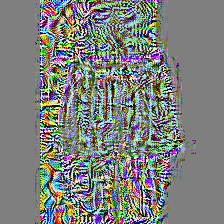
\includegraphics[width=3cm] {../thesis/images/adv/normal-24-epochs/cw/0.03/pertubation}};
\node [above=of pertubation, yshift=-1cm, color4, font=\small] {Pertubation};

\node [right=0.25cm of pertubation, inner sep=0.5pt, color3, font=\small] (equal) {$=$};

\node [rectangle, right=0.25cm of equal, inner sep=0.5pt, color3, draw, thick] (attack) {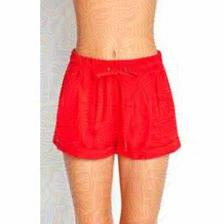
\includegraphics[width=3cm] {../thesis/images/adv/normal-24-epochs/cw/0.03/attack}};
\node [above=of attack, yshift=-1cm, color3, font=\small] {Adversarial};

\end{tikzpicture}
	\caption{Adversarial example, created using the \acs{CW} method with $\epsilon = 0.03$ and 1,000 iterations. The perturbation is normalized for visualization purposes.}
	\label{fig:cw-example}
\end{figure}
Cosine distance of feature vectors before and after attack:
\begin{align}
dist(\mathcal{F}(A),\,\mathcal{F}(T)) &= 0.6247 \\
dist(\mathcal{F}(A + \delta),\,\mathcal{F}(T)) &= 0.0049
\end{align}
Examining this one example, we can see that the achieved reduction in the cosine distance after the attack is even higher than in the case of \ac{PGD} and is therefore also high enough to successfully rank on the first place among the nearest neighbors of the target article, as seen in Figure~\ref{fig:cw-reco}. As seen in Table~\ref{tab:cw-results}, this first impression is confirmed once again when we evaluate the success rates achieved by \ac{CW} with 1,000 iterations on a broader set of attack tuples for $\epsilon$ values ranging from 0.01 to 0.05.
\begin{figure}[H]
	\centering
	\begin{tikzpicture}


\node [rectangle, inner sep=0.5pt, color1, draw, thick] (query) {\includegraphics[width=3cm] {../thesis/images/adv/target}};
\node [above=of query, yshift=-1cm, color1, font=\small] {\textbf{Query} image};


\node [right=of query.north east, rectangle, inner sep=0.5pt, color2, draw, thick] (orig1) {\includegraphics[width=2cm] {../../data/DeepFashion/img_resized/Mixed_Media_Knit_Tee/img_00000046.jpg}};
\node [above=of orig1, yshift=-1cm, color2, font=\small] {$dist = 0.0596$};

\node [right=0.5cm of orig1, rectangle, inner sep=0.5pt, color2, draw, thick] (orig2) {\includegraphics[width=2cm] {../../data/DeepFashion/img_resized/Striped_Boat_neck_Tee/img_00000088.jpg}};
\node [above=of orig2, yshift=-1cm, color2, font=\small] {$dist = 0.0615$};

\node [right=0.5cm of orig2, rectangle, inner sep=0.5pt, color2, draw, thick] (orig3) {\includegraphics[width=2cm] {../../data/DeepFashion/img_resized/Boat_Neck_Striped_Top/img_00000013.jpg}};
\node [above=of orig3, yshift=-1cm, color2, font=\small] {$dist = 0.0656$};

\node [right=0.5cm of orig3, rectangle, inner sep=0.5pt, color2, draw, thick] (orig4) {\includegraphics[width=2cm] {../../data/DeepFashion/img_resized/Nautical-Striped_Cotton_Tee/img_00000042.jpg}};
\node [above=of orig4, yshift=-1cm, color2, font=\small] {$dist = 0.0660$};


\node [right=of query.south east, rectangle, inner sep=0.5pt, color3, draw, thick] (adv1) {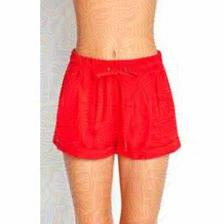
\includegraphics[width=2cm] {../thesis/images/adv/normal-24-epochs/cw/0.03/attack}};
\node [above=of adv1, yshift=-1cm, color3, font=\small] {$dist = 0.0049$};

\node [right=0.5cm of adv1, rectangle, inner sep=0.5pt, color3, draw, thick] (adv2) {\includegraphics[width=2cm] {../../data/DeepFashion/img_resized/Mixed_Media_Knit_Tee/img_00000046.jpg}};
\node [above=of adv2, yshift=-1cm, color3, font=\small] {$dist = 0.0596$};

\node [right=0.5cm of adv2, rectangle, inner sep=0.5pt, color3, draw, thick] (adv3) {\includegraphics[width=2cm] {../../data/DeepFashion/img_resized/Striped_Boat_neck_Tee/img_00000088.jpg}};
\node [above=of adv3, yshift=-1cm, color3, font=\small] {$dist = 0.0615$};

\node [right=0.5cm of adv3, rectangle, inner sep=0.5pt, color3, draw, thick] (adv4) {\includegraphics[width=2cm] {../../data/DeepFashion/img_resized/Boat_Neck_Striped_Top/img_00000013.jpg}};
\node [above=of adv4, yshift=-1cm, color3, font=\small] {$dist = 0.0656$};


\end{tikzpicture}
	\caption{Ranked recommendation results for original \acs{k-NN} index (top) and manipulated index with injected \acs{CW} adversarial example (bottom)}
	\label{fig:cw-reco}
\end{figure}
\begin{table}[H]
	\centering
	\begin{tabular}{ lccccc } 
		\toprule		
		& \multicolumn{5}{c}{Maximal Perturbation} \\
		\cmidrule{2-6}
		$rank_{min}$ & $\epsilon = 0.01$ & $\epsilon = 0.02$ & $\epsilon = 0.03$  & $\epsilon = 0.04$ & $\epsilon = 0.05$  \\
		\midrule
		1 & 74.60 & 94.10 & 96.40 & 97.60 & 97.80 \\
		3 & 83.10 & 98.10 & 99.40 & 99.70 & 99.70 \\
		10 & 86.60 & 98.40 & 99.50 & 99.90 & 99.90 \\
		100 & 91.30 & 99.40 & 99.90 & 100.00 & 100.00 \\
		\bottomrule
	\end{tabular}
	\caption{Success rates (\%) calculated over 1,000 random attack tuples using \acs{CW}-1000.}
	\label{tab:cw-results}
\end{table}
The maximum success rate for $rank_{min}=3$ achieved using \ac{CW} with 1,000 iterations in our experiments is 99.70\%, indicating that the more sophisticated approach of \ac{CW}, is indeed most effective at successfully finding worst-case perturbations that fulfill our adversary objective. When we look at the impact on the cosine distances in Figure~\ref{fig:cw-quantile}, we see a nearly perfect result. The vast majority of  points were successfully pushed onto the x-axis. Additionally, the spread of points along the y-axis is significantly narrower than in the case of \ac{PGD}, indicating a stronger and more reliable attack.
\begin{figure}[H]
	\centering
	% This file was created by tikzplotlib v0.9.3.
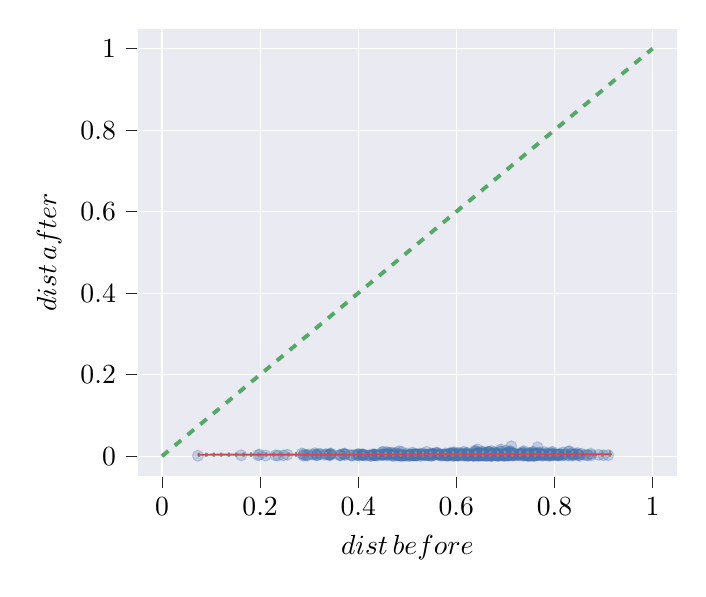
\begin{tikzpicture}

\definecolor{color0}{rgb}{0.917647058823529,0.917647058823529,0.949019607843137}
\definecolor{color1}{rgb}{0.298039215686275,0.447058823529412,0.690196078431373}
\definecolor{color2}{rgb}{0.768627450980392,0.305882352941176,0.32156862745098}
\definecolor{color3}{rgb}{0.333333333333333,0.658823529411765,0.407843137254902}

\begin{axis}[
axis background/.style={fill=color0},
axis line style={white},
tick align=outside,
tick pos=left,
x grid style={white},
xlabel={$dist\,before$},
xmajorgrids,
xmin=-0.05, xmax=1.05,
xtick style={color=white!15!black},
y grid style={white},
ylabel={$dist\,after$},
ymajorgrids,
ymin=-0.05, ymax=1.05,
ytick style={color=white!15!black}
]
\addplot [only marks, mark=*, draw=color1, fill=color1, opacity=0.25, colormap/blackwhite, clip marker paths=true]
table{%
	x                      y
	0.749930285186236 0.00514877492410959
	0.545129643540144 0.00455879661943648
	0.594492769416936 0.0060606506604165
	0.600027665432793 0.00402520929762551
	0.638901250457228 0.00376658193342339
	0.463720330028089 0.00373631873377456
	0.655212564656723 0.00286913458631166
	0.667302734936837 0.00994371252654236
	0.604248737557214 0.00336145074474947
	0.768675567754309 0.00505863273606311
	0.752788348234796 0.00565314795784133
	0.650282913752004 0.0048113205396797
	0.601176080609563 0.00223063704835058
	0.517418640449123 0.00459290083636454
	0.580926529019786 0.00184117961984598
	0.733954760471836 0.00325501123642735
	0.451353724135592 0.0107354958988978
	0.66267085109037 0.00230045313317628
	0.782254597504052 0.00226949586848169
	0.706724079843759 0.00859466956490451
	0.761523572340186 0.00384784776335978
	0.78926186224925 0.00107489982389575
	0.763543715079467 0.00541068235914122
	0.452488877660197 0.00304388956738466
	0.710497955045702 0.00671033104102048
	0.702901857887575 0.00451318616648932
	0.672992234181883 0.0015831655760471
	0.666921733101775 0.00330705748888061
	0.7566217800051 0.00512165066774151
	0.519871377234822 0.00426866491422728
	0.875197001576132 0.00226502818966801
	0.665647193644652 0.00321943402217073
	0.656419922116988 0.00229040482523435
	0.793901156253579 0.00565394830547472
	0.635987360711629 0.00368619278504356
	0.662296788673824 0.00130923168557806
	0.679245243974765 0.00375839290250779
	0.685393774907415 0.00262437291250661
	0.768680753516005 0.00259207062841616
	0.811280816403981 0.00531005826466002
	0.684760384108385 0.00253403461349266
	0.341904282690776 0.00361248031454153
	0.647352570807138 0.00625881873579592
	0.621504435491239 0.00586729322703228
	0.632745521528226 0.00545996125093917
	0.590320934346415 0.00371887204597476
	0.667024662712478 0.00411089766352402
	0.438489285799413 0.00160640606882434
	0.344277105227403 0.00625628696266323
	0.71699872156299 0.00632685926563159
	0.498407243330913 0.0021059514213515
	0.483467465917824 0.00642488614776171
	0.749213756359951 0.00456759967991016
	0.55368682979775 0.00277217086154047
	0.70436143717376 0.00283934593865121
	0.493354336297147 0.00202534883879668
	0.620492462672999 0.00254735031659326
	0.730098819559859 0.00225277640621124
	0.784399177470866 0.00552380371498085
	0.368801200721558 0.00528380554400776
	0.605573112358894 0.00351313490939298
	0.255697527237138 0.00368520287154361
	0.585480316600803 0.00673541993576832
	0.459824863338868 0.0024577533926482
	0.624803652334683 0.00227472018117236
	0.680977101938443 0.00723420842928002
	0.687925186136757 0.00262672496316463
	0.673318503485127 0.00319917170075157
	0.247373471137389 0.00209829455181609
	0.755410764220654 0.00597399726306236
	0.653689851164614 0.00335723910796892
	0.653369492588662 0.00995127602691948
	0.670459674172359 0.0049828078905878
	0.446337026680531 0.00461887184506704
	0.448592167369596 0.00977000787370241
	0.587242961968996 0.00396541654535798
	0.712916545072297 0.00489652968100929
	0.828198507673151 0.0110398797975034
	0.695538858955259 0.00216258612027331
	0.287937001678434 0.00137029155562962
	0.572467943893315 0.00276810623686086
	0.807446916651701 0.00273082492208399
	0.746712185561002 0.00206957534439889
	0.510824666414775 0.00235676058835743
	0.236535025206728 0.00161495038571569
	0.415833512457747 0.00170736975573271
	0.698159822893299 0.00325089081868202
	0.578022792131142 0.00673557865320484
	0.68907596182714 0.00480119177740002
	0.314826533337293 0.00427486588906201
	0.814141289737571 0.00436897859180885
	0.829855741223213 0.00148014072781033
	0.624752301751554 0.0030298297206478
	0.649136382485864 0.00704246589302759
	0.713177338051251 0.00452903548653483
	0.656059030199333 0.00646144540021476
	0.401925891795258 0.00152644232642918
	0.429227511345006 0.00467851260900176
	0.890072121308212 0.00324785404532957
	0.601583495523005 0.0018947930637534
	0.643290508808772 0.0165474699265464
	0.650941357374854 0.00277248061451507
	0.510177763137144 0.00337694927166932
	0.638454858460517 0.00953758207192879
	0.701349240321673 0.00647704023148854
	0.383878251541409 0.00277741626197825
	0.424993572022876 0.000950484554924191
	0.627088517501576 0.00434880888941591
	0.637760427938398 0.00431767016699613
	0.621689633278419 0.00341058281216211
	0.719092682452697 0.00349334210637808
	0.55269206398878 0.00622466094758412
	0.551854532751971 0.00397348496867989
	0.764876645750197 0.00318205406410665
	0.526247957392612 0.00494342231464295
	0.659319426942595 0.00392528602278386
	0.516423978851937 0.00230157241109208
	0.5837988257875 0.00283119068643434
	0.620100420885384 0.00347992354245552
	0.476709384823822 0.00792339855658086
	0.797959909520588 0.00549589912137272
	0.7149805335794 0.00137391009320187
	0.386458953919456 0.00129492326888736
	0.715513704514493 0.00619238913970599
	0.647599254705595 0.00592930844835082
	0.5622297493833 0.00358421512608131
	0.685895363941152 0.00333573830804712
	0.640932032441739 0.0058519564126428
	0.604813280230644 0.00229346315164869
	0.644703097247177 0.00314185544905454
	0.40062122760102 0.00268607827014999
	0.552930358347523 0.00280121039940029
	0.411959784933484 0.00294303018607267
	0.288898660519883 0.00478322292695821
	0.68862143996643 0.00561572812296196
	0.739151944950011 0.00573466415321067
	0.592411542529416 0.00122269480421133
	0.658491577506195 0.00296733634030621
	0.342519517304753 0.00509319476495063
	0.79532146294997 0.00410546946302581
	0.762028547338686 0.00506781882045904
	0.799270458852968 0.00321264089848494
	0.712060953415492 0.0242550761086326
	0.668421422269364 0.00256448528813913
	0.716270538034884 0.002588849912456
	0.736609850714618 0.00111168010347018
	0.71194978790719 0.0047414960861879
	0.817525668715114 0.00898101209804003
	0.538825044558296 0.00304069833816867
	0.616956697008118 0.003328827366052
	0.670440853181091 0.00106655193985628
	0.854951572643806 0.0057037080096205
	0.339905154035554 0.00347706353445676
	0.697012242102146 0.000940804146939311
	0.703934627680508 0.00593743470804331
	0.585150638018261 0.00219589921890218
	0.618183464409672 0.0033173393109287
	0.510580653153422 0.00885219377088653
	0.708204138546683 0.00246516812666186
	0.595116408822671 0.00175004786851785
	0.52953507124363 0.00317293866050661
	0.409222698617119 0.00342400057263437
	0.361546731401702 0.00263091701313412
	0.44534401863899 0.00261423644014403
	0.62868926769173 0.00253424523966572
	0.602092770821543 0.0054493800632982
	0.621731245740836 0.00639483443916267
	0.431986818536434 0.00299945276297853
	0.702221129987405 0.00264236052112399
	0.739681610939237 0.00266247286765009
	0.77478120202335 0.00145629832914929
	0.543598589615802 0.00163133456819953
	0.539491961514224 0.00281149474071218
	0.815559488540061 0.00172661128250895
	0.459091588651795 0.0100383007581005
	0.549477512109625 0.000772989361778831
	0.784411075838477 0.00265817261965395
	0.582495592527562 0.0025359081558709
	0.323674351889985 0.00464222317024232
	0.704530532048567 0.00417100546072757
	0.69920982381917 0.00484718623060376
	0.748899334871236 0.00559850894459413
	0.849871676841208 0.00296888839187703
	0.596532341602501 0.00931004844998917
	0.578612853508494 0.00269435658675199
	0.617463131279993 0.00243389877261557
	0.614893234844355 0.0107844402516606
	0.689595740143903 0.0121945941055298
	0.596387490096152 0.00208348670053105
	0.603793972670717 0.00239323977589534
	0.75869563111269 0.00430283108475926
	0.284846569743545 0.00633502849429479
	0.332399311344564 0.00378469947114679
	0.796633676144814 0.00267660024215588
	0.589232232903926 0.00633657664396203
	0.617920933934071 0.00322803492553791
	0.296423302496272 0.00181132165510411
	0.195767057352815 0.00235192540846252
	0.742647905333331 0.00211507216295514
	0.53571058262062 0.00380981310837536
	0.744356557181065 0.00184113587943235
	0.73323446206545 0.00601299562702451
	0.691536470137814 0.0106201912559183
	0.6777833959255 0.0100571648290891
	0.372449531923922 0.00600744329712732
	0.736675237111263 0.00398501988545252
	0.764965724837177 0.00237983614254234
	0.647264477347612 0.00192265057671082
	0.77175750809884 0.00468598183965141
	0.670207671613565 0.00440167765592847
	0.483185714582037 0.0120493126123273
	0.432773874473818 0.00306350549141765
	0.621400171354179 0.00834823104370497
	0.790122721483215 0.00201423105701792
	0.521317279069048 0.00320527056004449
	0.7178316986719 0.00409778029810215
	0.685656569607356 0.000702369848536555
	0.297906971254389 0.00370277218045656
	0.389515402074581 0.00236031449466645
	0.778480598364154 0.00190134122787555
	0.641682353591698 0.00277813730273813
	0.408557237591306 0.00329162791782456
	0.49406370150573 0.00135037931826587
	0.711865864883118 0.00369246615311036
	0.503247155318721 0.00321468042303097
	0.512894146507282 0.0024517606209542
	0.826518498710817 0.00273532517547626
	0.560593511402367 0.00678927933630646
	0.713108979779408 0.00494743670244979
	0.751605271430464 0.00188916194470423
	0.835447752792749 0.00669593059373697
	0.868038180167665 0.00290308518974636
	0.450759056338026 0.00460568620872648
	0.843768630019062 0.00389849336919912
	0.315878910242294 0.00215115217819484
	0.63360890721334 0.00161594290343403
	0.831832712922753 0.00486300649524995
	0.506923512324646 0.00450356148645137
	0.468339556190995 0.00353069070309542
	0.644477659171283 0.00794968876648738
	0.66798650155762 0.0013075961433956
	0.458159200201163 0.00397688928583084
	0.731185476860825 0.00600716031580151
	0.645236962485235 0.00197445596592905
	0.681812471427865 0.0047303104114349
	0.718586908546245 0.00492683275607908
	0.699917526819335 0.00170154989423899
	0.488549418874304 0.0104535880851986
	0.692466017003948 0.00261305914649468
	0.615908010896177 0.00160952224442268
	0.650035285113147 0.0016671382529293
	0.399011234951249 0.00421210648527626
	0.513861247185297 0.00184270632259231
	0.63537522120738 0.00251212949063928
	0.545364187962034 0.0031738126212556
	0.499585990046541 0.000965121794943902
	0.614519139294248 0.00205471733189233
	0.514931676841037 0.00413571155584047
	0.749234072134477 0.00272305526974459
	0.43118928131848 0.0026079405212901
	0.81958432613836 0.00417843453457711
	0.660807055360643 0.00258318154778858
	0.762737943939944 0.00513557933841202
	0.449584798894229 0.00325760810898079
	0.37267846638586 0.00534849562514705
	0.198980783261479 0.0039336175342185
	0.783055466861385 0.00676459960169973
	0.521357740491998 0.003421955647674
	0.315056542097085 0.00242194315639399
	0.458335868599957 0.00357803406771406
	0.757675846243778 0.0102333427563005
	0.549071355852816 0.00224739060954315
	0.709547602059916 0.00394974797141823
	0.681688309371418 0.00151002650418941
	0.231284867599328 0.00206081774446643
	0.61004094639827 0.0066531964379285
	0.211147031358891 0.00140340943743344
	0.759288978588741 0.00251248716017605
	0.409441611235067 0.00410507501373147
	0.515065587866478 0.00294315290964742
	0.641805529774103 0.0022908427805024
	0.801786004243514 0.00302819859351655
	0.595410632862571 0.00575930335389307
	0.532957351296172 0.00233343816765175
	0.775301148924077 0.0025085818524121
	0.770024582648653 0.00828518362981246
	0.670602879004158 0.00409687839777395
	0.710378535273008 0.00276704601245359
	0.768564306878313 0.00377260061141094
	0.589253706716992 0.00596229332432563
	0.396133176078856 0.00271211238476254
	0.0732170556102703 0.0010108204390552
	0.43481257794536 0.00260307975840324
	0.642169171952174 0.00622477872373139
	0.759650442139145 0.00172161894777079
	0.658041621190214 0.00136386287719448
	0.658704371445229 0.00495171150046358
	0.587385082874602 0.00331166881705103
	0.795722826403839 0.0108783082205363
	0.511139996236305 0.00317024686621636
	0.652898781957098 0.00221486682194583
	0.635549286038523 0.000892398105022729
	0.705919767362056 0.00170444550399351
	0.8377680849705 0.00321430319627225
	0.794675959384046 0.00451639665053827
	0.705369817117798 0.00233830536483837
	0.469346343833467 0.00205720389486008
	0.460755717852874 0.00724823477022607
	0.621511610559547 0.00194756944161711
	0.765596199364631 0.0218060403629084
	0.533333052028919 0.00582360335989385
	0.678229280021816 0.00671602570039909
	0.433663032745951 0.00421540902389783
	0.526893478723322 0.000940109466418426
	0.689078359479143 0.00341332519769255
	0.574756767799019 0.00289851809979591
	0.768349866288266 0.00823238552266936
	0.560135990570253 0.00875648644544558
	0.47829105197583 0.00337914724141553
	0.64252738384186 0.0056639621980793
	0.611059945959389 0.0036093645685924
	0.434091664969319 0.0028620389246089
	0.720103527792124 0.00424786930950516
	0.847461409085301 0.00757263187013457
	0.493629667723584 0.00275119072267038
	0.671369912402396 0.0122287625057739
	0.851265380003403 0.00103024799394169
	0.653498793335011 0.0105554831096395
	0.586328061611527 0.0037987470109242
	0.645866256662797 0.000762825556410607
	0.675124041643827 0.00234022614300578
	0.685767778149516 0.00151981221990893
	0.86729651523826 0.00194344641445166
	0.527626587013771 0.00611779233701537
	0.633819973628501 0.00232463456924736
	0.470825074131267 0.000523807307811652
	0.819603917614772 0.00278390096974501
	0.292770551751016 0.00188249859643486
	0.6639338355979 0.00745812530788148
	0.800849154684704 0.0043116742685676
	0.76081235083083 0.00298619517639687
	0.701126786202677 0.0135344800046608
	0.737464498407575 0.012321377699407
	0.363537414771168 0.00186490384781723
	0.426686420775209 0.00124844175403782
	0.489087655966448 0.000903314452819215
	0.670268744280959 0.00315417663785333
	0.505530253165333 0.00161963588877245
	0.740526225873231 0.00417944999246744
	0.899866196181995 0.00240704569486527
	0.483683264707208 0.00290264180291977
	0.449433361386744 0.00315281524440914
	0.746303976712037 0.00118367972588762
	0.750643758693575 0.00155724791296374
	0.612725974958442 0.0063696457149659
	0.59346940571212 0.00358058157337116
	0.544917278291259 0.00315226628525422
	0.728419301425855 0.00623549290444969
	0.764511254171688 0.00663698926512468
	0.70997086016244 0.0122303029485886
	0.512434430416371 0.00467778010235054
	0.626425312917439 0.00224296468059415
	0.671396688797416 0.00469307546478337
	0.660231987853023 0.00867791125999773
	0.693110582846953 0.00537214641159289
	0.567147231478984 0.00378194333596071
	0.587311375244521 0.00572759076325247
	0.618710172984232 0.00314702697618474
	0.515985522215755 0.00202787048279773
	0.609809931984589 0.0029114379171904
	0.694190835534683 0.0047627312231342
	0.421612967067194 0.00213222119527978
	0.804854826080207 0.00373985267523036
	0.81034806967294 0.00245918206275786
	0.400728662466072 0.0055888283594766
	0.68108993667488 0.0055485240275418
	0.624759536462276 0.00340621123172224
	0.639632643542499 0.00126762753993992
	0.565334451065483 0.00298487268837844
	0.724155973948268 0.00449060214637043
	0.780636445854131 0.00532334505164878
	0.688394234485562 0.00253156542341249
	0.717626048788916 0.00321193533404896
	0.794149961961326 0.00802258217081675
	0.653469196969942 0.00219397673837429
	0.583076179344785 0.00265597686252406
	0.662472973216852 0.00259567990903342
	0.745449476124617 0.00241211864027901
	0.678610291096507 0.00289118787390352
	0.625694597140793 0.00187256178221318
	0.406060771344487 0.00389431748882263
	0.476485971097163 0.00157343663898413
	0.468283805972484 0.00866467110999114
	0.634963852648431 0.00159503830684393
	0.837015416669889 0.00171587058878431
	0.642368123521645 0.00278889228336754
	0.739041424510359 0.00428335069692254
	0.845020498237548 0.00585249188831416
	0.656438355523641 0.0047566350901117
	0.515538564570085 0.00362750920795862
	0.639253538422845 0.00425386014183626
	0.755032018958287 0.0101802230820619
	0.650380370777574 0.00577743212761361
	0.595078914111771 0.00187448724308414
	0.736377011067756 0.0096784668754557
	0.638203687180116 0.0115117707532534
	0.576837682240758 0.00300328472382261
	0.73721716210528 0.00751618234189189
	0.67217652707097 0.000432427418539216
	0.576423060769707 0.00318859934504401
	0.807581171159848 0.00357485673624214
	0.551447881034208 0.00517053640951226
	0.748525874190978 0.00803122596510197
	0.804996102605875 0.00298053704382306
	0.596140818758331 0.00393128392959563
	0.848841393012694 0.00301205342644395
	0.522412467487752 0.00410312483824826
	0.708455471611262 0.0102090133483451
	0.655871650976444 0.00457733743866495
	0.344060300573647 0.00532598358649394
	0.550871513147255 0.00595401976959909
	0.793579360700296 0.00283805055204833
	0.307735583337964 0.00416061541633972
	0.760260452188501 0.00169393067747969
	0.679969271823598 0.00355723836829414
	0.161491432616658 0.00205868792231578
	0.539916291476205 0.0105158973548328
	0.793765993203607 0.00262827355541495
	0.485938274971863 0.00143919014036442
	0.709709732347336 0.0104415166614857
	0.520628779937858 0.00177174169831817
	0.754762385600963 0.000707102815157623
	0.571603682235088 0.00138856644128149
	0.518237726814111 0.00229775419557943
	0.592204071989852 0.00930383866881457
	0.831005373704125 0.0118338441284236
	0.475520197180245 0.0038208482632236
	0.535556359768757 0.00273735753065385
	0.48098746719898 0.00149864334654071
	0.643829596664848 0.00811028697225835
	0.69802747659834 0.00240753798506266
	0.662457590668849 0.00344732599435238
	0.761945984796663 0.00582956827848424
	0.673541753795479 0.00586875174944046
	0.599191071497787 0.00367193108068398
	0.583043355030542 0.00172641735172752
	0.861388372579893 0.00298946100980935
	0.909610467503274 0.00243221411504857
	0.757990551761491 0.0014418273364355
	0.75826993784914 0.00136006240084396
	0.571768528668209 0.0033010119494109
	0.645115377514972 0.00346938057279067
	0.690624358682331 0.0165630360314787
	0.640859499948553 0.00418253769348942
	0.657710850630101 0.0037095189682792
	0.684847926511692 0.00413403905805798
	0.543002375147646 0.00351782986669569
	0.334935754805303 0.00485598853231639
	0.410476630123713 0.00277832246986798
	0.580881766545294 0.0018340281089495
	0.485066486700019 0.00183110623716776
	0.464122371062565 0.0078354006798228
	0.311536427043663 0.00709894519019039
	0.60357763307252 0.00789503534756975
	0.567644206867215 0.00206452941341129
	0.78018159082219 0.00969077133652652
	0.750625788827556 0.00201519750311208
	0.602927392085652 0.00182945265569767
	0.560114475735146 0.00759089889790432
	0.645136885960052 0.00223266869388583
	0.66453546773761 0.0107239383120921
	0.725708373207391 0.00302080688384787
	0.701551621955118 0.00185681367099355
	0.60329022339761 0.00308470041801301
	0.431803054323183 0.00281001552730997
	0.633627568801737 0.00211641717583677
	0.643105758071873 0.00418752441125991
	0.666018860338931 0.0109126791848598
	0.488329713946807 0.0014367561043187
	0.713506163857739 0.00733729990145593
	0.838789537646401 0.00383813499112984
	0.563820743210674 0.00362616192243781
	0.363866719792442 0.00306985153213024
	0.623536798581518 0.00103294543140875
	0.638640031122458 0.0135375337611802
	0.738337916236993 0.00239040601766827
	0.726672985597008 0.00236061686003963
	0.498210973744068 0.00613442896278327
	0.790522605764815 0.00263519491037778
	0.706566038368266 0.00323352984771297
	0.504333978416028 0.00110350382959412
	0.660550712767169 0.00254072411005391
	0.774849612524017 0.003941383115866
	0.4388019804091 0.00239982762178026
	0.320376678990454 0.00600357992991685
	0.47188236732971 0.00648572658320812
	0.64695753561556 0.00496251380014467
	0.543728043609814 0.0036661751896031
	0.808275522011065 0.00375475825699967
	0.506634973765494 0.00201049963724864
	0.661000170829586 0.00159589930232917
	0.874513143513846 0.0058778978995303
	0.695563916037077 0.00192309022111981
	0.606108998274253 0.00220780390478692
	0.74767255304931 0.0010824648830674
	0.722919974255095 0.00316943669707836
	0.3428549213663 0.00222063557842689
	0.672602020253343 0.00220957655485821
	0.807176195809274 0.00197359790376939
	0.373006429550312 0.00321593860460856
	0.665290882404377 0.00245255964226931
	0.697525868126369 0.00331448386228306
};
\addplot [line width=0.7pt, white!54.9019607843137!black, dotted]
table {%
	0.0732170556102703 0.00110093694714916
	0.166988139897396 0.0011289481415232
	0.260759224184521 0.00115695933589723
	0.354530308471647 0.00118497053027127
	0.448301392758772 0.0012129817246453
	0.542072477045898 0.00124099291901934
	0.635843561333023 0.00126900411339337
	0.729614645620149 0.00129701530776741
	0.823385729907274 0.00132502650214144
	0.9171568141944 0.00135303769651548
};
\addplot [line width=0.7pt, white!54.9019607843137!black, dotted]
table {%
	0.0732170556102703 0.001546902867944
	0.166988139897396 0.00161151946878103
	0.260759224184521 0.00167613606961807
	0.354530308471647 0.0017407526704551
	0.448301392758772 0.00180536927129214
	0.542072477045898 0.00186998587212917
	0.635843561333023 0.00193460247296621
	0.729614645620149 0.00199921907380324
	0.823385729907274 0.00206383567464028
	0.9171568141944 0.00212845227547731
};
\addplot [line width=0.7pt, white!54.9019607843137!black, dotted]
table {%
	0.0732170556102703 0.00208325004884095
	0.166988139897396 0.00213115767465728
	0.260759224184521 0.0021790653004736
	0.354530308471647 0.00222697292628992
	0.448301392758772 0.00227488055210625
	0.542072477045898 0.00232278817792257
	0.635843561333023 0.00237069580373889
	0.729614645620149 0.00241860342955522
	0.823385729907274 0.00246651105537154
	0.9171568141944 0.00251441868118786
};
\addplot [line width=0.7pt, white!54.9019607843137!black, dotted]
table {%
	0.0732170556102703 0.00265886745882164
	0.166988139897396 0.00267933395527034
	0.260759224184521 0.00269980045171905
	0.354530308471647 0.00272026694816776
	0.448301392758772 0.00274073344461647
	0.542072477045898 0.00276119994106517
	0.635843561333023 0.00278166643751388
	0.729614645620149 0.00280213293396259
	0.823385729907274 0.00282259943041129
	0.9171568141944 0.00284306592686
};
\addplot [line width=0.7pt, white!54.9019607843137!black, dotted]
table {%
	0.0732170556102703 0.00320330428838803
	0.166988139897396 0.00320573946097938
	0.260759224184521 0.00320817463357074
	0.354530308471647 0.00321060980616209
	0.448301392758772 0.00321304497875345
	0.542072477045898 0.0032154801513448
	0.635843561333023 0.00321791532393616
	0.729614645620149 0.00322035049652751
	0.823385729907274 0.00322278566911887
	0.9171568141944 0.00322522084171022
};
\addplot [line width=0.7pt, white!54.9019607843137!black, dotted]
table {%
	0.0732170556102703 0.00354673492624768
	0.166988139897396 0.00358162320886875
	0.260759224184521 0.00361651149148982
	0.354530308471647 0.0036513997741109
	0.448301392758772 0.00368628805673197
	0.542072477045898 0.00372117633935304
	0.635843561333023 0.00375606462197411
	0.729614645620149 0.00379095290459518
	0.823385729907274 0.00382584118721625
	0.9171568141944 0.00386072946983732
};
\addplot [line width=0.7pt, white!54.9019607843137!black, dotted]
table {%
	0.0732170556102703 0.00370542296979397
	0.166988139897396 0.0038069782123073
	0.260759224184521 0.00390853345482063
	0.354530308471647 0.00401008869733396
	0.448301392758772 0.00411164393984728
	0.542072477045898 0.00421319918236061
	0.635843561333023 0.00431475442487394
	0.729614645620149 0.00441630966738726
	0.823385729907274 0.00451786490990059
	0.9171568141944 0.00461942015241392
};
\addplot [line width=0.7pt, white!54.9019607843137!black, dotted]
table {%
	0.0732170556102703 0.00432855261599905
	0.166988139897396 0.00449314900998215
	0.260759224184521 0.00465774540396526
	0.354530308471647 0.00482234179794836
	0.448301392758772 0.00498693819193147
	0.542072477045898 0.00515153458591457
	0.635843561333023 0.00531613097989768
	0.729614645620149 0.00548072737388078
	0.823385729907274 0.00564532376786389
	0.9171568141944 0.00580992016184699
};
\addplot [line width=0.7pt, white!54.9019607843137!black, dotted]
table {%
	0.0732170556102703 0.00532771616562089
	0.166988139897396 0.00551770204410563
	0.260759224184521 0.00570768792259037
	0.354530308471647 0.0058976738010751
	0.448301392758772 0.00608765967955984
	0.542072477045898 0.00627764555804458
	0.635843561333023 0.00646763143652932
	0.729614645620149 0.00665761731501405
	0.823385729907274 0.00684760319349879
	0.9171568141944 0.00703758907198353
};
\addplot [line width=0.7pt, white!54.9019607843137!black, dotted]
table {%
	0.0732170556102703 0.00620728107728038
	0.166988139897396 0.00681345536928092
	0.260759224184521 0.00741962966128145
	0.354530308471647 0.00802580395328199
	0.448301392758772 0.00863197824528253
	0.542072477045898 0.00923815253728307
	0.635843561333023 0.00984432682928361
	0.729614645620149 0.0104505011212841
	0.823385729907274 0.0110566754132847
	0.9171568141944 0.0116628497052852
};
\addplot [line width=0.7pt, color2]
table {%
	0.0732170556102703 0.00351826825452184
	0.166988139897396 0.00364545297573133
	0.260759224184521 0.00377263769694082
	0.354530308471647 0.0038998224181503
	0.448301392758772 0.00402700713935979
	0.542072477045898 0.00415419186056928
	0.635843561333023 0.00428137658177876
	0.729614645620149 0.00440856130298825
	0.823385729907274 0.00453574602419774
	0.9171568141944 0.00466293074540723
};
\addplot [line width=1.4pt, color3, dashed]
table {%
	0 0
	1 1
};
\end{axis}

\end{tikzpicture}

	\caption{Quantile regression plot of 512 sampled cosine distances between target and attack article, before and after performing \acs{CW}-1000 attacks, using $\epsilon=0.05$}
	\label{fig:cw-quantile}
\end{figure}
\subsection{Comparison}
Finally, we want to compare the achieved results of all evaluated attack methods. An overview of the different attack success rates for a minimum target rank of 3 or lower is shown in Table~\ref{tab:attack-results} and Figure~\ref{fig:top3-normal-success}.  Looking at the results, \ac{PGD} and \ac{CW} achieve remarkably high success rates going up to 99.70\%. \ac{FGSM}, on the other hand, achieved insufficient results and was not able to achieve our adversary objective. When attacking an undefended model, the performance increase of \ac{CW}-1000 compared to \ac{PGD}-128 is relatively small and arguably not worth the extra computational cost (approx. $\times 7.5$), which the significantly more complex attack method requires. Therefore we consider \ac{PGD}-128 as the best trade-off between attack strength and computational cost.

\begin{table}[H]
	\centering
	\begin{tabular}{ lccccc } 
		\toprule		
		& \multicolumn{5}{c}{Maximal Perturbation} \\
		\cmidrule{2-6}
		Attack & $\epsilon = 0.01$ & $\epsilon = 0.02$ & $\epsilon = 0.03$  & $\epsilon = 0.04$ & $\epsilon = 0.05$  \\
		\midrule
		FGSM & 0.27 & 0.16 & 0.14 & 0.09 & 0.07 \\
		PGD-8 & 22.19 & 36.40 & 35.60 & 32.41 & 27.95 \\
		PGD-16 & 33.36 & 64.28 & 72.95 & 74.06 & 72.69 \\
		PGD-32 & 40.93 & 78.95 & 88.85 & 91.80 & 92.78 \\
		PGD-64 & 44.33 & 86.40 & 94.06 & 96.13 & 97.09 \\
		PGD-128 & 45.92 & 89.79 & 96.33 & 97.69 & 98.32 \\
		CW-1000 & 83.10 & 98.10 & 99.40 & 99.70 & 99.70 \\
		\bottomrule
	\end{tabular}
	\caption{Success rates (\%) for $rank_{min}=3$, calculated over 10,000 random article tuples (1,000 in the case of \acs{CW}) for all evaluated attacks and $\epsilon$ values.}
	\label{tab:attack-results}
\end{table}

\begin{figure}[H]
	\centering
	% This file was created by tikzplotlib v0.9.3.
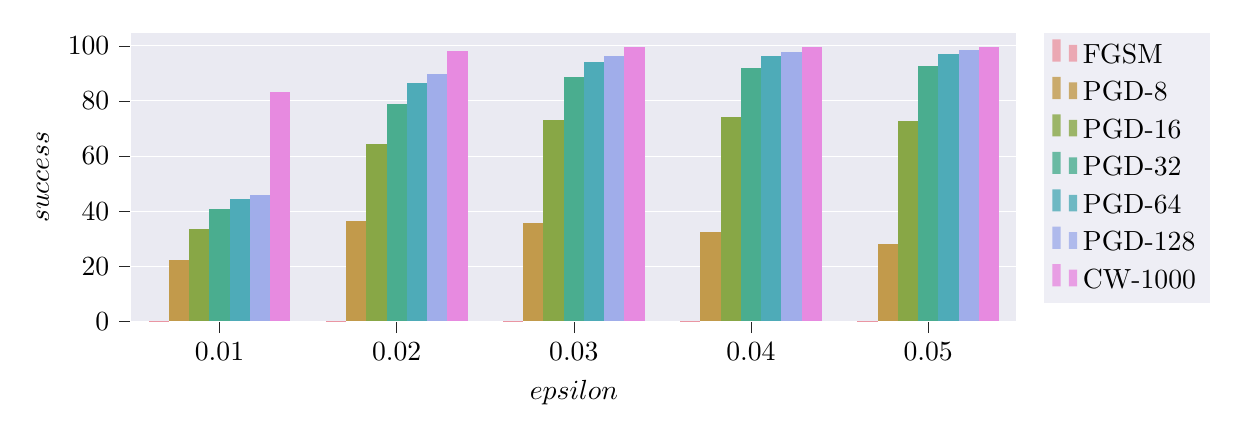
\begin{tikzpicture}

\definecolor{color0}{rgb}{0.917647058823529,0.917647058823529,0.949019607843137}
\definecolor{color1}{rgb}{0.916118471592631,0.587423760636183,0.640263770354658}
\definecolor{color2}{rgb}{0.761932343861879,0.602524817229626,0.29239128864167}
\definecolor{color3}{rgb}{0.531977299570092,0.653932867339067,0.275419601514511}
\definecolor{color4}{rgb}{0.289388368632853,0.678978856556939,0.561244957348417}
\definecolor{color5}{rgb}{0.307108018655975,0.671626456963976,0.723521305871116}
\definecolor{color6}{rgb}{0.626885214598887,0.677767791860435,0.916300649166299}
\definecolor{color7}{rgb}{0.90409992612099,0.540448897448067,0.880107767162344}

\begin{axis}[
axis background/.style={fill=color0},
axis line style={white},
legend pos = outer north east,
legend cell align={left},
legend style={row sep=1.2pt, fill opacity=0.8, draw opacity=0, text opacity=1, draw=none, fill=color0},
tick align=outside,
tick pos=left,
x=2.25cm,
y=0.035cm,
x grid style={white},
xlabel={$epsilon$},
xmin=-0.5, xmax=4.5,
xtick style={color=white!15!black},
xtick={0,1,2,3,4},
xticklabels={0.01,0.02,0.03,0.04,0.05},
y grid style={white},
ylabel={$success$},
ymajorgrids,
ymin=0, ymax=104.685,
ytick style={color=white!15!black}
]
\draw[draw=none,fill=color1,line width=0.12pt] (axis cs:-0.4,0) rectangle (axis cs:-0.285714285714286,0.27);
\addlegendimage{ybar,ybar legend,draw=none,fill=color1,line width=0.12pt};
\addlegendentry{FGSM}

\draw[draw=none,fill=color1,line width=0.12pt] (axis cs:0.6,0) rectangle (axis cs:0.714285714285714,0.16);
\draw[draw=none,fill=color1,line width=0.12pt] (axis cs:1.6,0) rectangle (axis cs:1.71428571428571,0.14);
\draw[draw=none,fill=color1,line width=0.12pt] (axis cs:2.6,0) rectangle (axis cs:2.71428571428571,0.09);
\draw[draw=none,fill=color1,line width=0.12pt] (axis cs:3.6,0) rectangle (axis cs:3.71428571428571,0.07);
\draw[draw=none,fill=color2,line width=0.12pt] (axis cs:-0.285714285714286,0) rectangle (axis cs:-0.171428571428571,22.19);
\addlegendimage{ybar,ybar legend,draw=none,fill=color2,line width=0.12pt};
\addlegendentry{PGD-8}

\draw[draw=none,fill=color2,line width=0.12pt] (axis cs:0.714285714285714,0) rectangle (axis cs:0.828571428571429,36.4);
\draw[draw=none,fill=color2,line width=0.12pt] (axis cs:1.71428571428571,0) rectangle (axis cs:1.82857142857143,35.6);
\draw[draw=none,fill=color2,line width=0.12pt] (axis cs:2.71428571428571,0) rectangle (axis cs:2.82857142857143,32.41);
\draw[draw=none,fill=color2,line width=0.12pt] (axis cs:3.71428571428571,0) rectangle (axis cs:3.82857142857143,27.95);
\draw[draw=none,fill=color3,line width=0.12pt] (axis cs:-0.171428571428571,0) rectangle (axis cs:-0.0571428571428571,33.36);
\addlegendimage{ybar,ybar legend,draw=none,fill=color3,line width=0.12pt};
\addlegendentry{PGD-16}

\draw[draw=none,fill=color3,line width=0.12pt] (axis cs:0.828571428571429,0) rectangle (axis cs:0.942857142857143,64.28);
\draw[draw=none,fill=color3,line width=0.12pt] (axis cs:1.82857142857143,0) rectangle (axis cs:1.94285714285714,72.95);
\draw[draw=none,fill=color3,line width=0.12pt] (axis cs:2.82857142857143,0) rectangle (axis cs:2.94285714285714,74.06);
\draw[draw=none,fill=color3,line width=0.12pt] (axis cs:3.82857142857143,0) rectangle (axis cs:3.94285714285714,72.69);
\draw[draw=none,fill=color4,line width=0.12pt] (axis cs:-0.0571428571428571,0) rectangle (axis cs:0.0571428571428571,40.93);
\addlegendimage{ybar,ybar legend,draw=none,fill=color4,line width=0.12pt};
\addlegendentry{PGD-32}

\draw[draw=none,fill=color4,line width=0.12pt] (axis cs:0.942857142857143,0) rectangle (axis cs:1.05714285714286,78.95);
\draw[draw=none,fill=color4,line width=0.12pt] (axis cs:1.94285714285714,0) rectangle (axis cs:2.05714285714286,88.85);
\draw[draw=none,fill=color4,line width=0.12pt] (axis cs:2.94285714285714,0) rectangle (axis cs:3.05714285714286,91.8);
\draw[draw=none,fill=color4,line width=0.12pt] (axis cs:3.94285714285714,0) rectangle (axis cs:4.05714285714286,92.78);
\draw[draw=none,fill=color5,line width=0.12pt] (axis cs:0.0571428571428571,0) rectangle (axis cs:0.171428571428571,44.33);
\addlegendimage{ybar,ybar legend,draw=none,fill=color5,line width=0.12pt};
\addlegendentry{PGD-64}

\draw[draw=none,fill=color5,line width=0.12pt] (axis cs:1.05714285714286,0) rectangle (axis cs:1.17142857142857,86.4);
\draw[draw=none,fill=color5,line width=0.12pt] (axis cs:2.05714285714286,0) rectangle (axis cs:2.17142857142857,94.06);
\draw[draw=none,fill=color5,line width=0.12pt] (axis cs:3.05714285714286,0) rectangle (axis cs:3.17142857142857,96.13);
\draw[draw=none,fill=color5,line width=0.12pt] (axis cs:4.05714285714286,0) rectangle (axis cs:4.17142857142857,97.09);
\draw[draw=none,fill=color6,line width=0.12pt] (axis cs:0.171428571428571,0) rectangle (axis cs:0.285714285714286,45.92);
\addlegendimage{ybar,ybar legend,draw=none,fill=color6,line width=0.12pt};
\addlegendentry{PGD-128}

\draw[draw=none,fill=color6,line width=0.12pt] (axis cs:1.17142857142857,0) rectangle (axis cs:1.28571428571429,89.79);
\draw[draw=none,fill=color6,line width=0.12pt] (axis cs:2.17142857142857,0) rectangle (axis cs:2.28571428571429,96.33);
\draw[draw=none,fill=color6,line width=0.12pt] (axis cs:3.17142857142857,0) rectangle (axis cs:3.28571428571429,97.69);
\draw[draw=none,fill=color6,line width=0.12pt] (axis cs:4.17142857142857,0) rectangle (axis cs:4.28571428571429,98.32);
\draw[draw=none,fill=color7,line width=0.12pt] (axis cs:0.285714285714286,0) rectangle (axis cs:0.4,83.1);
\addlegendimage{ybar,ybar legend,draw=none,fill=color7,line width=0.12pt};
\addlegendentry{CW-1000}

\draw[draw=none,fill=color7,line width=0.12pt] (axis cs:1.28571428571429,0) rectangle (axis cs:1.4,98.1);
\draw[draw=none,fill=color7,line width=0.12pt] (axis cs:2.28571428571429,0) rectangle (axis cs:2.4,99.4);
\draw[draw=none,fill=color7,line width=0.12pt] (axis cs:3.28571428571429,0) rectangle (axis cs:3.4,99.7);
\draw[draw=none,fill=color7,line width=0.12pt] (axis cs:4.28571428571429,0) rectangle (axis cs:4.4,99.7);
\addplot [line width=1.26pt, white!26!black, forget plot]
table {%
	-0.342857142857143 nan
	-0.342857142857143 nan
};
\addplot [line width=1.26pt, white!26!black, forget plot]
table {%
	0.657142857142857 nan
	0.657142857142857 nan
};
\addplot [line width=1.26pt, white!26!black, forget plot]
table {%
	1.65714285714286 nan
	1.65714285714286 nan
};
\addplot [line width=1.26pt, white!26!black, forget plot]
table {%
	2.65714285714286 nan
	2.65714285714286 nan
};
\addplot [line width=1.26pt, white!26!black, forget plot]
table {%
	3.65714285714286 nan
	3.65714285714286 nan
};
\addplot [line width=1.26pt, white!26!black, forget plot]
table {%
	-0.228571428571429 nan
	-0.228571428571429 nan
};
\addplot [line width=1.26pt, white!26!black, forget plot]
table {%
	0.771428571428571 nan
	0.771428571428571 nan
};
\addplot [line width=1.26pt, white!26!black, forget plot]
table {%
	1.77142857142857 nan
	1.77142857142857 nan
};
\addplot [line width=1.26pt, white!26!black, forget plot]
table {%
	2.77142857142857 nan
	2.77142857142857 nan
};
\addplot [line width=1.26pt, white!26!black, forget plot]
table {%
	3.77142857142857 nan
	3.77142857142857 nan
};
\addplot [line width=1.26pt, white!26!black, forget plot]
table {%
	-0.114285714285714 nan
	-0.114285714285714 nan
};
\addplot [line width=1.26pt, white!26!black, forget plot]
table {%
	0.885714285714286 nan
	0.885714285714286 nan
};
\addplot [line width=1.26pt, white!26!black, forget plot]
table {%
	1.88571428571429 nan
	1.88571428571429 nan
};
\addplot [line width=1.26pt, white!26!black, forget plot]
table {%
	2.88571428571429 nan
	2.88571428571429 nan
};
\addplot [line width=1.26pt, white!26!black, forget plot]
table {%
	3.88571428571429 nan
	3.88571428571429 nan
};
\addplot [line width=1.26pt, white!26!black, forget plot]
table {%
	0 nan
	0 nan
};
\addplot [line width=1.26pt, white!26!black, forget plot]
table {%
	1 nan
	1 nan
};
\addplot [line width=1.26pt, white!26!black, forget plot]
table {%
	2 nan
	2 nan
};
\addplot [line width=1.26pt, white!26!black, forget plot]
table {%
	3 nan
	3 nan
};
\addplot [line width=1.26pt, white!26!black, forget plot]
table {%
	4 nan
	4 nan
};
\addplot [line width=1.26pt, white!26!black, forget plot]
table {%
	0.114285714285714 nan
	0.114285714285714 nan
};
\addplot [line width=1.26pt, white!26!black, forget plot]
table {%
	1.11428571428571 nan
	1.11428571428571 nan
};
\addplot [line width=1.26pt, white!26!black, forget plot]
table {%
	2.11428571428571 nan
	2.11428571428571 nan
};
\addplot [line width=1.26pt, white!26!black, forget plot]
table {%
	3.11428571428571 nan
	3.11428571428571 nan
};
\addplot [line width=1.26pt, white!26!black, forget plot]
table {%
	4.11428571428571 nan
	4.11428571428571 nan
};
\addplot [line width=1.26pt, white!26!black, forget plot]
table {%
	0.228571428571429 nan
	0.228571428571429 nan
};
\addplot [line width=1.26pt, white!26!black, forget plot]
table {%
	1.22857142857143 nan
	1.22857142857143 nan
};
\addplot [line width=1.26pt, white!26!black, forget plot]
table {%
	2.22857142857143 nan
	2.22857142857143 nan
};
\addplot [line width=1.26pt, white!26!black, forget plot]
table {%
	3.22857142857143 nan
	3.22857142857143 nan
};
\addplot [line width=1.26pt, white!26!black, forget plot]
table {%
	4.22857142857143 nan
	4.22857142857143 nan
};
\addplot [line width=1.26pt, white!26!black, forget plot]
table {%
	0.342857142857143 nan
	0.342857142857143 nan
};
\addplot [line width=1.26pt, white!26!black, forget plot]
table {%
	1.34285714285714 nan
	1.34285714285714 nan
};
\addplot [line width=1.26pt, white!26!black, forget plot]
table {%
	2.34285714285714 nan
	2.34285714285714 nan
};
\addplot [line width=1.26pt, white!26!black, forget plot]
table {%
	3.34285714285714 nan
	3.34285714285714 nan
};
\addplot [line width=1.26pt, white!26!black, forget plot]
table {%
	4.34285714285714 nan
	4.34285714285714 nan
};
\end{axis}

\end{tikzpicture}

	\caption{Success rates (\%) for $rank_{min}=3$, calculated over 10,000 random article tuples (1,000 in the case of \acs{CW}) for all evaluated attacks and $\epsilon$ values.}
	\label{fig:top3-normal-success}
\end{figure}

\subsection{Classifier Impact}
An interesting observation we made during our experiments, is that the performed attacks on the cosine distance of image embeddings also indirectly attack the classifier, which was initially trained in Chapter~\ref{chp:model}. By minimizing the cosine distance between two articles, the predictions of the classifier for these articles also become more similar, as seen in Figure~\ref{fig:classifier-attack}.
\begin{figure}
	\centering
	\subfloat[][Target image with ground-truth labels: $category = Sweater$, $texture = stripe$.]{
		\includegraphics[width=0.25\textwidth]{images/adv/target}
	}\hspace{0.5cm}
	\subfloat[][Original image with ground-truth labels: $category = Shorts$, $texture = linen$.]{
		\includegraphics[width=0.25\textwidth]{images/adv/original}
	}\hspace{0.5cm}
	\subfloat[][Adversarial image, created using \ac{PGD} with 32 iterations and $\epsilon=0.03$.]{					
		\includegraphics[width=0.25\textwidth]{images/adv/normal-24-epochs/pgd/0.03/attack}
	}\\
	\subfloat[][Classifier predictions for category and texture of target image.]{
		\begin{tikzpicture}
\begin{groupplot}[group style={group size=2 by 1, horizontal sep=2.5cm}, width=5.5cm]

\nextgroupplot[
axis background/.style={fill=color0},
axis line style={white},
legend cell align={left},
legend style={fill opacity=0.8, draw opacity=1, text opacity=1, at={(0.03,0.97)}, anchor=north west, draw=none, fill=color0, font=\scriptsize},
tick align=outside,
tick pos=left,
xmajorgrids,
scaled x ticks = false, 
scaled y ticks = false, 
x grid style={white},
y grid style={white},
ymajorgrids,
xtick style={color=white!15!black},
ytick style={color=white!15!black},
ticklabel style = {font=\scriptsize},
title={Category: Tee},
xmin=0, xmax=0.535,
ymin=-0.25, ymax=10.15,
ytick={0.375,...,10.375},
yticklabels={Dress, Tank, Shorts, Henley, Cardigan, Hoodie, Blouse, Top, Sweater, Tee}
]

\draw[draw=none,fill=color1] (axis cs:0,0) rectangle (axis cs:0.0031,0.75);
\draw[draw=none,fill=color1] (axis cs:0,1) rectangle (axis cs:0.0054,1.75);
\draw[draw=none,fill=color1] (axis cs:0,2) rectangle (axis cs:0.0059,2.75);
\draw[draw=none,fill=color1] (axis cs:0,3) rectangle (axis cs:0.0163,3.75);
\draw[draw=none,fill=color1] (axis cs:0,4) rectangle (axis cs:0.0169,4.75);
\draw[draw=none,fill=color1] (axis cs:0,5) rectangle (axis cs:0.0173,5.75);
\draw[draw=none,fill=color1] (axis cs:0,6) rectangle (axis cs:0.0371,6.75);
\draw[draw=none,fill=color1] (axis cs:0,7) rectangle (axis cs:0.1207,7.75);
\draw[draw=none,fill=color2] (axis cs:0,8) rectangle (axis cs:0.2472,8.75);
\draw[draw=none,fill=color1] (axis cs:0,9) rectangle (axis cs:0.5157,9.75);

\nextgroupplot[
axis background/.style={fill=color0},
axis line style={white},
legend cell align={left},
legend style={fill opacity=0.8, draw opacity=1, text opacity=1, at={(0.03,0.97)}, anchor=north west, draw=none, fill=color0, font=\scriptsize},
tick align=outside,
tick pos=left,
xmajorgrids,
scaled x ticks = false, 
scaled y ticks = false, 
x grid style={white},
y grid style={white},
ymajorgrids,
xtick style={color=white!15!black},
ytick style={color=white!15!black},
ticklabel style = {font=\scriptsize},
title={Texture: striped},
xmin=0, xmax=0.47,
ymin=-0.25, ymax=10.15,
ytick={0.375,...,10.375},
yticklabels={nautical stripe, print, stripes, nautical, marled, nautical striped, breton stripe, breton, stripe, striped}
]

\draw[draw=none,fill=color1] (axis cs:0,0) rectangle (axis cs:0.0112,0.75);
\draw[draw=none,fill=color1] (axis cs:0,1) rectangle (axis cs:0.0113,1.75);
\draw[draw=none,fill=color1] (axis cs:0,2) rectangle (axis cs:0.0180,2.75);
\draw[draw=none,fill=color1] (axis cs:0,3) rectangle (axis cs:0.0208,3.75);
\draw[draw=none,fill=color1] (axis cs:0,4) rectangle (axis cs:0.0211,4.75);
\draw[draw=none,fill=color1] (axis cs:0,5) rectangle (axis cs:0.0219,5.75);
\draw[draw=none,fill=color1] (axis cs:0,6) rectangle (axis cs:0.0250,6.75);
\draw[draw=none,fill=color1] (axis cs:0,7) rectangle (axis cs:0.0453,7.75);
\draw[draw=none,fill=color2] (axis cs:0,8) rectangle (axis cs:0.1997,8.75);
\draw[draw=none,fill=color1] (axis cs:0,9) rectangle (axis cs:0.4596,9.75);
\end{groupplot}

\end{tikzpicture}

	}\\
	\subfloat[][Classifier predictions for category and texture of original image.]{
		\begin{tikzpicture}
\begin{groupplot}[group style={group size=2 by 1, horizontal sep=2.5cm}, width=5.5cm]

\nextgroupplot[
axis background/.style={fill=color0},
axis line style={white},
legend cell align={left},
legend style={fill opacity=0.8, draw opacity=1, text opacity=1, at={(0.03,0.97)}, anchor=north west, draw=none, fill=color0, font=\scriptsize},
tick align=outside,
tick pos=left,
xmajorgrids,
scaled x ticks = false, 
scaled y ticks = false, 
x grid style={white},
y grid style={white},
ymajorgrids,
xtick style={color=white!15!black},
ytick style={color=white!15!black},
ticklabel style = {font=\scriptsize},
title={Category: Shorts},
xmin=0, xmax=1.0,
ymin=-0.25, ymax=10.15,
ytick={0.375,...,10.375},
yticklabels={Blouse, Joggers, Top, Leggings, Culottes, Sweatshorts, Cutoffs, Skirt, Trunks, Shorts}
]

\draw[draw=none,fill=color1] (axis cs:0,0) rectangle (axis cs:1.8125e-06,0.75);
\draw[draw=none,fill=color1] (axis cs:0,1) rectangle (axis cs:2.8439e-06,1.75);
\draw[draw=none,fill=color1] (axis cs:0,2) rectangle (axis cs:1.1450e-05,2.75);
\draw[draw=none,fill=color1] (axis cs:0,3) rectangle (axis cs:2.1354e-05,3.75);
\draw[draw=none,fill=color1] (axis cs:0,4) rectangle (axis cs:2.3611e-05,4.75);
\draw[draw=none,fill=color1] (axis cs:0,5) rectangle (axis cs:8.1404e-05,5.75);
\draw[draw=none,fill=color1] (axis cs:0,6) rectangle (axis cs:0.0002,6.75);
\draw[draw=none,fill=color1] (axis cs:0,7) rectangle (axis cs:0.0003,7.75);
\draw[draw=none,fill=color1] (axis cs:0,8) rectangle (axis cs:0.0222,8.75);
\draw[draw=none,fill=color2] (axis cs:0,9) rectangle (axis cs:0.9772,9.75);

\nextgroupplot[
axis background/.style={fill=color0},
axis line style={white},
legend cell align={left},
legend style={fill opacity=0.8, draw opacity=1, text opacity=1, at={(0.03,0.97)}, anchor=north west, draw=none, fill=color0, font=\scriptsize},
tick align=outside,
tick pos=left,
xmajorgrids,
scaled x ticks = false, 
scaled y ticks = false, 
x grid style={white},
y grid style={white},
ymajorgrids,
xtick style={color=white!15!black},
ytick style={color=white!15!black},
ticklabel style = {font=\scriptsize},
title={Texture: print},
xmin=0, xmax=0.227,
ymin=-0.25, ymax=10.15,
ytick={0.375,...,10.375},
yticklabels={floral print, pom-pom, tribal, stripe, printed, polka dot, dot, floral, striped, print}
]

\draw[draw=none,fill=color1] (axis cs:0,0) rectangle (axis cs:0.0214,0.75);
\draw[draw=none,fill=color1] (axis cs:0,1) rectangle (axis cs:0.0237,1.75);
\draw[draw=none,fill=color1] (axis cs:0,2) rectangle (axis cs:0.0342,2.75);
\draw[draw=none,fill=color1] (axis cs:0,3) rectangle (axis cs:0.0507,3.75);
\draw[draw=none,fill=color1] (axis cs:0,4) rectangle (axis cs:0.0668,4.75);
\draw[draw=none,fill=color1] (axis cs:0,5) rectangle (axis cs:0.0741,5.75);
\draw[draw=none,fill=color1] (axis cs:0,6) rectangle (axis cs:0.0823,6.75);
\draw[draw=none,fill=color1] (axis cs:0,7) rectangle (axis cs:0.0834,7.75);
\draw[draw=none,fill=color1] (axis cs:0,8) rectangle (axis cs:0.0878,8.75);
\draw[draw=none,fill=color1] (axis cs:0,9) rectangle (axis cs:0.2200,9.75);
\end{groupplot}

\end{tikzpicture}

	}\\
	\subfloat[][Classifier predictions for category and texture of adversarial image.]{
		\begin{tikzpicture}
\begin{groupplot}[group style={group size=2 by 1, horizontal sep=2.5cm}, width=5.5cm]

\nextgroupplot[
axis background/.style={fill=color0},
axis line style={white},
legend cell align={left},
legend style={fill opacity=0.8, draw opacity=1, text opacity=1, at={(0.03,0.97)}, anchor=north west, draw=none, fill=color0, font=\scriptsize},
tick align=outside,
tick pos=left,
xmajorgrids,
scaled x ticks = false, 
scaled y ticks = false, 
x grid style={white},
y grid style={white},
ymajorgrids,
xtick style={color=white!15!black},
ytick style={color=white!15!black},
ticklabel style = {font=\scriptsize},
title={Category: Top},
xmin=0, xmax=0.32,
ymin=-0.25, ymax=10.15,
ytick={0.375,...,10.375},
yticklabels={Dress, Skirt, Shorts, Tank, Hoodie, Cardigan, Blouse, Tee, Sweater, Top}
]

\draw[draw=none,fill=color1] (axis cs:0,0) rectangle (axis cs:0.0067,0.75);
\draw[draw=none,fill=color1] (axis cs:0,1) rectangle (axis cs:0.0091,1.75);
\draw[draw=none,fill=color2] (axis cs:0,2) rectangle (axis cs:0.0114,2.75);
\draw[draw=none,fill=color1] (axis cs:0,3) rectangle (axis cs:0.0127,3.75);
\draw[draw=none,fill=color1] (axis cs:0,4) rectangle (axis cs:0.0219,4.75);
\draw[draw=none,fill=color1] (axis cs:0,5) rectangle (axis cs:0.0599,5.75);
\draw[draw=none,fill=color1] (axis cs:0,6) rectangle (axis cs:0.0847,6.75);
\draw[draw=none,fill=color1] (axis cs:0,7) rectangle (axis cs:0.2071,7.75);
\draw[draw=none,fill=color3] (axis cs:0,8) rectangle (axis cs:0.2579,8.75);
\draw[draw=none,fill=color1] (axis cs:0,9) rectangle (axis cs:0.3113,9.75);

\nextgroupplot[
axis background/.style={fill=color0},
axis line style={white},
legend cell align={left},
legend style={fill opacity=0.8, draw opacity=1, text opacity=1, at={(0.03,0.97)}, anchor=north west, draw=none, fill=color0, font=\scriptsize},
tick align=outside,
tick pos=left,
xmajorgrids,
scaled x ticks = false, 
scaled y ticks = false, 
x grid style={white},
y grid style={white},
ymajorgrids,
xtick style={color=white!15!black},
ytick style={color=white!15!black},
ticklabel style = {font=\scriptsize},
title={Texture: striped},
xmin=0, xmax=0.525,
ymin=-0.25, ymax=10.15,
ytick={0.375,...,10.375},
yticklabels={mixed, abstract, polka dot, dot, linen, nautical, stripes, print, stripe, striped}
]

\draw[draw=none,fill=color1] (axis cs:0,0) rectangle (axis cs:0.0111,0.75);
\draw[draw=none,fill=color1] (axis cs:0,1) rectangle (axis cs:0.0112,1.75);
\draw[draw=none,fill=color1] (axis cs:0,2) rectangle (axis cs:0.0115,2.75);
\draw[draw=none,fill=color1] (axis cs:0,3) rectangle (axis cs:0.0136,3.75);
\draw[draw=none,fill=color2] (axis cs:0,4) rectangle (axis cs:0.0137,4.75);
\draw[draw=none,fill=color1] (axis cs:0,5) rectangle (axis cs:0.0237,5.75);
\draw[draw=none,fill=color1] (axis cs:0,6) rectangle (axis cs:0.0240,6.75);
\draw[draw=none,fill=color1] (axis cs:0,7) rectangle (axis cs:0.0265,7.75);
\draw[draw=none,fill=color3] (axis cs:0,8) rectangle (axis cs:0.1615,8.75);
\draw[draw=none,fill=color1] (axis cs:0,9) rectangle (axis cs:0.5098,9.75);
\end{groupplot}

\end{tikzpicture}

	}
	\caption{\acs{k-NN} attacks indirectly attack classifier.}
	\label{fig:classifier-attack}
\end{figure}
